
\documentclass[11pt,fleqn]{article}
\usepackage[margin=1in,top=1in,bottom=1in]{geometry}
\usepackage{mathtools}
\usepackage{longtable}
\usepackage{enumitem}
\usepackage{hyperref}
\usepackage[dvips]{graphics}
\usepackage[table]{xcolor}
\usepackage{amssymb}
\usepackage{subfig}
\usepackage{booktabs}
\usepackage{tikz}

\usepackage[normalem]{ulem}

\usepackage{multicol}
\usepackage{txfonts}
%\usepackage{amsfonts}
\usepackage{natbib}

\usepackage{gb4e}
%\usepackage{/Users/judith/Library/Latex/drs}
%\usepackage{/Users/judith/Library/Latex/avm}
\usepackage[all]{xy}
\usepackage{rotating}
\usepackage{tipa}
\usepackage{multirow}
\usepackage{authblk}
\usepackage{adjustbox}
\usepackage{array}


\newcolumntype{R}[2]{%
    >{\adjustbox{angle=#1,lap=\width-(#2)}\bgroup}%
    l%
    <{\egroup}%
}
\newcommand*\rot{\multicolumn{1}{R{60}{1em}}}% no optional argument here, please!

\newcommand{\foc}{$_{\mbox{\small F}}$}
\newcommand{\lp}{<_{\hspace*{-.1cm}p}}
\newcommand{\lnai}{<_{\hspace*{-.1cm}nai}}

\setlength{\parindent}{.8cm}
\setlength{\parskip}{0ex}
\setlength{\headsep}{0in}

\setlength{\bibsep}{0mm}
\bibpunct[:]{(}{)}{;}{a}{,}{,}

\newcommand{\yi}{\'{\symbol{16}}}
\newcommand{\nasi}{\~{\symbol{16}}}
\newcommand{\hina}{h\nasi na}
\newcommand{\ina}{\nasi na}
%\renewcommand{\abut}{$\supset$\hspace*{-0.07cm}$\subset$}
\newcommand{\tto}{t$_{top}$}
\newcommand{\wtop}{w$_{top}$}
\newcommand{\tc}{t$_c$}
\newcommand{\schwa}{\begin{sideways}e\end{sideways}}

% Semantic brackets
%\newcommand{\iss}[1]{\mbox{\protect\tiny \mbox{#1}}}
%\newcommand{\sem}[2]{\6#1\9$_\iss{#2}$} David's original
\newcommand{\6}{\mbox{$[\hspace*{-.6mm}[$}} 
\newcommand{\9}{\mbox{$]\hspace*{-.6mm}]$}}
\newcommand{\sem}[2]{\6#1\9$^{#2}$}

\newcommand{\semt}[2]{$\left[\hspace*{-.6mm}\left[\begin{tabular}[c]{@{}l@{}}#1\vspace*{-.5em}\end{tabular}\right]\hspace*{-.6mm}\right]\hspace*{-.6mm}^{#2}$}

\renewcommand{\baselinestretch}{1}

\def\bad{{\leavevmode\llap{*}}}
\def\marginal{{\leavevmode\llap{?}}}
\def\verymarginal{{\leavevmode\llap{??}}}
\def\infelic{{\leavevmode\llap{\#}}}

\definecolor{Lighter}{gray}{.92}
\definecolor{Blue}{RGB}{0,0,255}
\definecolor{Green}{RGB}{10,200,100}
\definecolor{Red}{RGB}{255,0,0}


\newcommand{\citepos}[1]{\citeauthor{#1}'s \citeyear{#1}}
\newcommand{\citeposs}[1]{\citeauthor{#1}'s}
\newcommand{\citetpos}[1]{\citeauthor{#1}'s (\citeyear{#1})}

\newcommand{\eref}[1]{(\ref{#1})}
\newcommand{\tableref}[1]{Table \ref{#1}}
\newcommand{\figref}[1]{Fig.~\ref{#1}}
\newcommand{\appref}[1]{Appendix \ref{#1}}
\newcommand{\sectionref}[1]{Section \ref{#1}}


\title{At-issueness predicts projection variability\thanks{Discussions with Craige Roberts and Mandy Simons have greatly influenced our thinking about projective content and the research reported on in this paper over the years. For helpful feedback, we also thank M\'arta Abrus\'an, audiences at many universities and conferences since 2015, as well as David Barner and three anonymous reviewers of {\em Journal of Semantics}. This work was partially supported by NSF grants BCS-1452674 (JT) and BCS-1452663 (DIB).}}

\author[$\bullet$]{Judith Tonhauser}
\author[$\triangleright$]{Judith Degen}
\author[$\circ$]{David I.\ Beaver}

\affil[$\bullet$]{The Ohio State University}
\affil[$\triangleright$]{Stanford University}
\affil[$\circ$]{University of Texas at Austin}

\renewcommand\Authands{ and }

\newcommand{\jt}[1]{\textbf{\color{blue}JT: #1}}
\newcommand{\jd}[1]{\textbf{\color{Green}[jd: #1]}}  

\begin{document}

\maketitle

\begin{abstract}
Projective content is utterance content that a speaker may be taken to be committed to even when the expression associated with the content occurs embedded under an entailment-canceling operator (e.g., \citealt{ccmg90}). It has long been observed that projective content varies in how robustly it projects (e.g., \citealt{karttunen71b,simons01,abusch10}), though preliminary experimental research has been able to confirm only some of the intuitions about projection variability (e.g., \citealt{xue-onea11,smith-hall11}). Given the sparse empirical evidence for projection variability, the first goal of this paper was to investigate projection variability for projective content associated with 19 expressions of American English. The second goal was to explore the hypothesis that the projectivity of projective content is a function of its at-issueness (\citealt{brst-salt10,brst-ar}); according to this hypothesis, called the `Projection Principle', variable at-issueness is implicated in projection variability. The findings of two pairs of experiments provide robust empirical evidence for projection variability and for the Projection Principle. We show that many analyses of projection  cannot account for the observed projection variability and discuss the implications of our finding that projective content varies in its at-issueness for an empirically adequate analysis of projection.

\end{abstract}

%\tableofcontents

%\newpage
			
\section{Introduction}\label{s1}

Projective content is utterance content that the speaker may be taken to be committed to even when the expression associated with the content occurs in the syntactic scope of an entailment-canceling operator (see, e.g., \citealt{ccmg90}). To illustrate, consider the examples in (\ref{eng1}) and (\ref{eng2}). Since (\ref{eng1}) entails the content of the complement of {\em discover}, that Mike visited Alcatraz, the speaker of (\ref{eng1}) is taken to be committed to this content. The so-called Family-of-Sentences variants of (\ref{eng1}) given in (\ref{eng2}a-d) do not entail this content because {\em discover} is embedded under entailment-canceling operators: negation in (\ref{eng2}a), the polar question operator in (\ref{eng2}b), the epistemic possibility modal {\em perhaps} in (\ref{eng2}c) and the antecedent of a conditional in (\ref{eng2}d). Since speakers who utter the sentences in (\ref{eng2}a-d) may nevertheless be taken to be committed to the content of the complement, this content, by virtue of being able to `project' over the entailment-canceling operators, is considered projective content. 

\begin{exe}
\ex\label{eng1}  Felipe discovered that Mike visited Alcatraz.

\ex\label{eng2}
\begin{xlist} 
\ex Felipe didn't discover that Mike visited Alcatraz.
\ex Did Felipe discover that Mike visited Alcatraz?
\ex Perhaps Felipe discovered that Mike visited Alcatraz.
\ex If Felipe discovered that Mike visited Alcatraz, he'll get mad.
\end{xlist}
\end{exe}

Why does projective content project? One of the most successful and widely adopted answers to this question is that projective content is conventionally specified to project, for instance, by being required to be entailed by or satisfied in the common ground of the interlocutors (e.g., \citealt{heim83,vds92,geurts99}). On such `conventionalist' approaches, the lexical entry of {\em discover} specifies that the content of its clausal complement is required to be entailed by or satisfied in the common ground of the interlocutors, thereby ensuring that the speaker is taken to be committed to the content. Since conventionalist approaches only distinguish projective and non-projective content, such approaches are challenged by the long-standing observation that some projective content projects less robustly than other such content. In the early 1970s already, \citet{karttunen71b} pointed out that the content of the complement of {\em regret} in (\ref{semi-factive}a) is more robustly projective than the content of the complement of {\em discover} in (\ref{semi-factive}b); following \citealt{karttunen71b}, predicates like {\em discover} have been referred to as `semi-factive', in contrast to their `factive' counterparts like {\em regret} (and `non-factive' predicates like {\em believe}). \citet{schlenker10} referred to the predicate {\em announce} as a `part-time trigger' because the content of its complement may, but often does not, project.

\begin{exe}
\ex\label{semi-factive}
\begin{xlist}
\ex John didn't discover that he had not told the truth.  
\ex John didn't regret that he had not told the truth.
\hfill (\citealt[63]{karttunen71b})

\end{xlist}
\end{exe}

Similarly, \citet[432]{simons01} noted, partially based on examples from \citealt{ccmg90} and \citealt{geurts94}, that the projection of ``some -- but crucially, not all'' projective content to the common ground of the interlocutors may be suppressed in explicit ignorance contexts. Example (\ref{hardsoft}a), for instance, shows that the projective content associated with {\em win} in the antecedent of the conditional, that John participated in the race, need not be part of the common ground of the interlocutors, i.e., need not project. On the other hand, the existential implication of the cleft in (\ref{hardsoft}b), that there is an individual who read the letter, must be part of the common ground of the interlocutors, i.e., must project. Expressions like {\em win} are referred to as `soft triggers', in contrast to `hard triggers', like the cleft (see also, e.g., \citealt{abusch10,abrusan2016}).\footnote{In this paper, we do not use the term `trigger' to refer to expressions associated with projective content since this term evokes conventional theories of projection. To remain neutral about how projective content comes to be projective, we instead use `expression associated with projective content'.}

\begin{exe}
\ex\label{hardsoft}
\begin{xlist}

\ex I have no idea whether John ended up participating in the Road Race yesterday. But if he won it, then he has more victories than anyone else in history. \hfill (\citealt[39]{abusch10})

\ex\infelic I have no idea whether anyone read that letter. But if it is John
who read it, let's ask him to be discreet about the content. \hfill (\citealt[40]{abusch10})

\end{xlist}
\end{exe}

Experimental research has provided preliminary evidence for projection variability. \citet{xue-onea11} observed that the content of the complement of German {\em wissen} `know' is less projective than the content of the complement of {\em erfahren} `find out', both of which are less projective than the relevant projective contents of sentences with {\em auch} `too' (that a parallel event is contextually salient) and {\em wieder} `again' (that the relevant event has happened before). Similarly, \citet{smith-hall11} found that the projective contents of {\em win} and {\em know} are less projective than the content implication of English definite noun phrases (e.g., for {\em the queen}, that the referent is a queen). Interestingly, they also found that the existential implication of cleft sentences, considered a hard trigger, was (numerically) less projective than the relevant contents of the soft triggers {\em win} and {\em know}. Thus, the sparse experimental evidence confirms some but not all of the intuitions about projection variability reported in the literature.\footnote{Projection variability is also reported in experimental research that did not investigate such variability. In \citealt{just-clark1973}, the projective content associated with the negative predicates {\em forget} and {\em to be thoughtless}, embedded in the antecedent of a conditional, took longer to verify than that of the positive predicates {\em remember} and {\em to be thoughtful}, respectively. In \citealt{harris1974}, the extent to which the projective content associated with eight change of state predicates and motion verbs embedded under negation was judged to be true was reported to be variable. In \citealt{harris1974b}, the content of the complement of `factive' predicates was found to be more projective than the content of the complement of `non-factive' predicates. Finally, \citet{tiemann-etal11} noted that projective content differs in how acceptable it was judged in contexts that did not entail the relevant content.}

Observations about projection variability challenge any approach to projection that does not offer an explanation for why some projective content seems to systematically project less robustly than other such content. Under conventionalist approaches, for instance, the lexical specifications of expressions like {\em regret, discover, win}, clefts and definite noun phrases predict that their relevant contents can project, but do not predict differences in how robustly the contents project. And although the process of local accommodation allows conventionalist approaches to capture that a particular utterance content does not project to the common ground of the interlocutors, this process is not understood well-enough to capture systematic differences between projective contents associated with distinct expressions. Thus, referring to expressions associated with projective content as `semi-factive' or `soft', as opposed to `factive' or `hard', provides a way of pigeon-holing projectively variable constructions, but does not address the challenge that this variability poses for conventionalist approaches to projection.  Given the sparse empirical evidence for projection variability, a first goal of this paper is to explore projection variability for a broad range of projective content, to better understand the extent to which projective content varies in projectivity. 

One possible explanation for projection variability is that projectivity derives from a property that projective content shares, but shares to varying degrees. \citet{brst-salt10} proposed that `at-issueness' is implicated in projectivity (see also \citealt{abrusan2011}), i.e., the ability of content to address the Question Under Discussion (QUD; e.g., \citealt{roberts12}).  Specifically, Simons and her colleagues proposed that utterance content projects if and only if it is not at-issue with respect to the QUD addressed by the utterance. This hypothesis was formulated as the Projection Principle in \citealt[280]{brst-ar}:\footnote{According to \citealt[315]{brst-salt10}, there is a causal relation between projection and at-issueness: utterance content projects not just {\em when} but {\em because} it is not-at-issue. The Projection Principle as formulated in \citealt{brst-ar} is neutral about whether not-at-issueness causes projection or whether not-at-issueness is merely correlated with projection. The experiments we report on here were designed to test the Projection Principle, i.e., whether not-at-issueness is correlated with projection. We leave the question of whether there is a causal relationship between not-at-issueness and projection to future research. We also note that the Projection Principle is compatible with conventional and pragmatic approaches to how projective content arises in the first place. We return to the implications of our findings for analyses of projective content and projection in section \ref{s5}.}

\begin{exe}
\ex\label{pp} {\bf Projection Principle:} If content $C$ is expressed by a constituent embedded under an entailment-canceling operator, then $C$ projects if and only if $C$ is not at-issue.

\end{exe} 
To illustrate the Projection Principle, consider the question-answer pairs in (\ref{nrrc}). The example in (\ref{nrrc}a) shows that the content of the NRRC in B's utterance cannot be used to address A's question, and hence is not at-issue;\footnote{\citet{syrett-koev2015} show that the content of NRRCs can be the target of direct denial, which may be taken to suggest that this content can be at-issue. We return to this matter in section \ref{s-disc2}.} the example in (\ref{nrrc}b), on the other hand, shows that the main clause content of B's utterance can address A's question and hence is at-issue. The Projection Principle consequently predicts that the content of the NRRC projects from B's utterance in (\ref{nrrc}b) whereas the content of the main clause does not project. 

\begin{exe}
\ex\label{nrrc}
\begin{xlist}
\ex
\begin{xlist}
\exi{A:} Did Mike visit Alcatraz?
\exi{B:} \infelic Mike, who visited Alcatraz, is interested in the history of prisons.
\end{xlist}


\ex
\begin{xlist}
\exi{A:} What is Mike interested in?
\exi{B:} Mike, who visited Alcatraz, is interested in the history of prisons.
\end{xlist}

\end{xlist}
\end{exe}

Simons and her colleagues did not consider that projective content varies in how robustly it projects.

projection variability, the Projection Principle predicts such variability. It predicts, for instance, that the content of non-restrictive relative clauses (NRRCs) projects more robustly, by virtue of being not at-issue (\citealt{potts05}), than the content of the complement of {\em discover}, which can be at-issue and not-at-issue (\citealt{simons07}). Consider the question-answer pairs in (\ref{nrrc}). 

 The content of the complement of {\em discover}, on the other hand, can be not-at-issue, as shown in (\ref{discover}a), but it can also be at-issue, as shown in (\ref{discover}b). 


\begin{exe}
\ex\label{discover}
\begin{xlist}

\ex
\begin{xlist}
\exi{A:} Why is Henry in such a bad mood?
\exi{B:} He discovered that Harriet had a job interview at Princeton. 
\end{xlist}

\ex
\begin{xlist}
\exi{A:} Where was Harriet yesterday?
\exi{B:} Henry discovered that she had a job interview at Princeton. \hfill (\citealt[1035]{simons07})
\end{xlist}
\end{xlist}
\end{exe}
Thus, the Projection Principle predicts that if the content of NRRCs is more robustly not-at-issue than the content of the complement of {\em discover}, the former projects more robustly than the latter. As summarized in (\ref{questions}), the second goal of this paper is to test the Projection Principle:

\begin{exe}
\ex\label{questions} {\bf Research questions}

\begin{xlist} 

\ex Does projective content vary in how robustly it projects?

\ex Is projectivity a function of at-issueness, as predicted by the Projection Principle?
\end{xlist}

\end{exe} 

The two research questions in (\ref{questions}) are explored in this paper on the basis of two pairs of experiments, which jointly serve to identify empirical generalizations that an empirically adequate analysis of projection needs to account for. In exploring the first research question (Exps.~1a and 1b), we expand on and improve on previous experimental research on projection variability. In \citealt{xue-onea11} and \citealt{smith-hall11}, projection variability was explored for 4 German and 6 English expressions associated with projective content, respectively. Exps.~1a and 1b significantly broaden our understanding of projection variability by considering the projective content associated with 19 expressions. 

Our experiments also take into consideration that world knowledge may influence projection: a speaker might, for instance, be more likely to be taken to be committed to a content describing an event of Alexander flying to New York than to a content describing an event of Alexander flying to the moon, simply because people are more likely to fly to New York than the moon. Thus, whether projective content projects may depend on the prior probability of the event described by lexical content,\footnote{World knowledge as encoded in prior probabilities of different parts of the meaning space has been shown to affect interpretation in ways captured by models of language use that treat interpretation as Bayesian reasoning about an observed utterance (see, e.g., \citealt{frankejaeger2016, goodmanfrank2016}).} such that content that describes more a priori likely event may be more likely to project. If this is right, then, for example, the content of the clausal complement of {\em Did Bill discover that Alexander flew to New York?} should be more likely to project than that of {\em Did Bill discover that Alexander flew to the moon?}. 

In this paper, we do not systematically manipulate the prior probabilities of events, but we do introduce event-type variability by including lexical contents that describe a wide variety of events. In our experiments, these lexical contents instantiate the projective contents associated with expressions like {\em discover}. In the remainder of the paper, the term `lexical content' refers to the description of a particular event and the term `projective content' refers to an abstract characterization of the projective content associated with an expression. For instance, in  a sentence like {\em Did Bill discover that Alexander flew to New York?}, the relevant expression is {\em discover}, the projective content is the content of its clausal complement, and the lexical content (of the projective content) describes the event of Alexander flying to New York.  Thus, our experiments consider that the lexical content that instantiates projective content may matter for how robustly the projective content is taken to be a commitment of the speaker and how likely the projective content is to address the QUD. The projective content associated with the 6 expressions explored in \citealt{smith-hall11} was only instantiated by one lexical content each and a distinct lexical content instantiated each projective content. Our experiments, in contrast, included a total of 37 lexical contents and the projective content associated with each expression was instantiated by up to 20 lexical contents. Furthermore, to facilitate comparison across different projective contents and the expressions associated with the projective content, the projective contents of distinct expressions were instantiated with the same lexical contents: overall, each of the 37 lexical contents instantiated up to 12 projective contents.

Our research on the second research question also builds on and significantly expands previous experimental work. 
 Using a direct dissent diagnostic for at-issueness, \citet{amaral-etal11} found that speakers of British English judged direct dissent with the projective content associated with {\em only} (the prejacent) to be more acceptable than direct dissent with the projective content associated with {\em continue} and {\em stop} (the pre- and post-state implications, respectively). These findings suggest that the prejacent of {\em only} is more at-issue than the post- and pre-state implications of {\em continue} and {\em stop}, respectively. (See also \citealt{cummins-etal2012}, and \citealt{amaral-cummins2015} for similar results on Spanish.) \citet{xue-onea11} found that speakers of German were more likely to directly dissent with the content of the complement of {\em wissen} `know' than with the content of the complement of {\em erfahren} `find out' and, in turn, more likely to directly dissent with these contents than with projective contents of {\em auch} `too' and {\em wieder} again'. These results suggest that the projective content associated with {\em wissen} `know' is more at-issue than the projective content associated with {\em erfahren} `find out', which in turn is comparatively more at-issue than the projective contents associated with {\em auch} `too' and {\em wieder} again'. Interestingly, comparing the relative projectivity and not-at-issueness 
of the projective contents across their two experiments, \citet[180]{xue-onea11} point to ``a clear correlation between projection and not-at-issueness'', in line with the Projection Principle. Our Exps.~1a and 1b improve on \citetpos{xue-onea11} study by exploring the projectivity and at-issueness of projective content as within-item and within-participant factors. The design of these experiments therefore allows us to quantify the correlation between not-at-issueness and projectivity, and to consider by-item and by-participant variability. 

The diagnostics for at-issueness employed in the literature rely on different assumptions about how at-issue and not-at-issue content are distinguished. In Exps.~1a and 1b, we rely on a diagnostic that assumes that the context set is more likely to be partitioned by at-issue content and its negation, than by not-at-issue content and its negation. For other applications of diagnostics that rely on this assumption see, e.g., \citealt{amaral-etal07} and \citealt{tonhauser-sula6}. To make sure that the at-issueness results in Exps.~1 are not just an artifact of the at-issueness diagnostic used, a second pair of experiments, Exps.~2a and 2b, explore the at-issueness of the projective contents of the first pair of experiments, Exps.~1a and 1b, using a different diagnostic for at-issueness. Specifically, the diagnostic used in Exps.~2a and 2b relies on the assumption that at-issue and not-at-issue content differ in the extent to which it is up for debate and can be directly assented/dissented with. For previous uses of diagnostics that rely on this assumption see, e.g., \citealt{amaral-etal07,xue-onea11,murray2014,anderbois-etal2015,destruel-etal2015,tonhauser-sula6} and \citealt{syrett-koev2015}. We return to the issue of adequately operationalizing at-issueness below. 

The paper proceeds as follows. In section \ref{s2}, we characterize the projective contents explored in this paper. Section \ref{s3} addresses the two goals of the paper on the basis of Exps.~1a and 1b, and section \ref{s4} extends our investigation of the second goal on the basis of Exps.~2a and 2b. In section \ref{s5}, we discuss the implications of our findings for analyses of projection. Section \ref{s6} concludes the paper.


\section{The projective contents explored in the experiments}\label{s2}

The two pairs of experiments explore the projective contents associated with 19 target expressions. The projective content associated with the 9 target expressions in Exp.~1a are syntactically heterogeneous, as shown in (\ref{pairs1a2a}), whereas the 12 target expressions included in Exp.~1b are all (semi-)factive attitude predicates, as shown in (\ref{pairs1b2b}). Since some expressions can contribute multiple projective contents (\citealt{brst-lang11}), we specify, for each target expression, the projective content investigated in our experiments: e.g., in (\ref{pairs1a2a}a), `sentence-medial NRRCs' identifies the target expression and `content of the NRRC' identifies the projective content. For the syntactically heterogeneous target expressions in (\ref{pairs1a2a}), a sample sentence illustrating the expression is provided and the corresponding projective content is identified. Exps.~2a and 2b explored not-at-issueness for the same expression/projective content pairs as Exps.~1a and 1b, respectively. Since the projective content associated with the attitude predicates {\em is annoyed} and {\em discovered} was explored in both pairs of experiments, a total of 19 expression/projective content pairs were explored. 

\begin{exe}
\ex\label{pairs1a2a} {\bf Target expression / projective content pairs in Experiments 1a and 2a}

\begin{enumerate}[itemsep=-.5mm]

\item Sentence-medial NRRCs / content of the NRRC
\\ e.g., {\em These muffins, which have blueberries in them, are gluten-free and low-fat.} / `These muffins have blueberries in them.'

\item Sentence-medial nominal appositives / appositive content
\\ e.g., {\em Martha's new car, a BMW, was expensive.} / `Martha's new car is a BMW'

\item Posessive noun phrases / possession implication
\\ e.g., {\em Martha's new BMW was expensive.} / `Martha's new car is a BMW'

\item {\em be annoyed} / content of the clausal complement
\\ e.g., {\em Martha's neighbor is annoyed that Martha has a new BMW.} / `Martha has a new BMW'

\item {\em discover} / content of the clausal complement
\\ e.g., {\em Mary discovered that her daughter has been biting her nails.} / `Mary's daughter has been biting her nails'

\item {\em know} / content of the clausal complement
\\ e.g., {\em Billy knows that Martha has a new BMW.} /  `Martha has a new BMW'

\item {\em only} / prejacent
\\ e.g., {\em These muffins only have blueberries in them.} / `These muffins have blueberries in them'

\item {\em stop} / pre-state implication
\\ e.g., {\em Mary's daughter stopped biting her nails.}  / `Mary's daughter has been biting her nails'

\item {\em be stupid to} / prejacent
\\ e.g., {\em Mary's daughter is stupid to be biting her nails.} / `Mary's daughter has been biting her nails'

\end{enumerate}


\ex\label{pairs1b2b} {\bf Target expressions in Experiments 1b and 2b; the associated projective content was the content of the clausal complement}

{\em be amused, be annoyed, be aware, see, discover, find out, notice, realize, learn, establish, confess, reveal} 

\end{exe}

In what follows, we characterize the properties of the 19 target expression/projective content pairs explored in the experiments.

\paragraph{Projectivity} The 19 projective contents share the property of being projective, i.e., being able to be taken to be a commitment of the speaker even when the expression that the projective content is associated with is embedded under an entailment-canceling operator. The 9 expressions included in Experiments 1a and 2a differ in how robustly their contents have been reported to project: 
the relevant contents of NRRCs, nominal appositives and of the emotive `factive' predicate {\em annoyed} are typically taken to project more robustly than, e.g., the prejacent of {\em only}, the pre-state implication of {\em stop} and the complement of the cognitive `semi-factive' predicate {\em discover} (e.g., \citealt{karttunen71b,simons01,potts05,abusch10,beaver-belly}). The 12 target expressions included in Experiments 1b and 2b include both `factive' and `semi-factive' predicates, and were also chosen to denote different types of attitudes: emotive predicates ({\em be amused, be annoyed}), cognitive predicates ({\em be aware, discover, find out, notice, realize, learn, establish}), sensory predicates ({\em see}) and communication predicates ({\em confess, reveal}). The predicates {\em be annoyed} and {\em discover} were included in both Exps.~1a and 1b (and 2a and 2b) to be able to directly compare the results of the experiments.

\paragraph{Strong Contextual Felicity} A property shared by the 19 target expression/projective content pairs is that they do not impose a Strong Contextual Felicity constraint on the utterance context (\citealt{brst-lang11}). What this means is that utterances with the target expressions are judged to be acceptable in contexts in which the projective content is not already part of the common ground of the interlocutors when the expression is uttered (i.e., the projective content is not anaphoric). For instance, B's utterance in (\ref{nrrc}b), repeated below, is acceptable even if A did not previously know the content of the NRRC, that Mike visited Alcatraz. An expression/projective content pair that is associated with a Strong Contextual Felicity constraint is the pronoun {\em they} and the projective content that there is a uniquely salient plurality of individuals (to which the pronoun refers). Use of {\em they} in (\ref{scf}) is judged to be unacceptable because the projective content associated with the pronoun is not part of the common ground of the interlocutors, i.e., the utterance context does not entail the existence of a uniquely salient plurality of individuals to which the pronoun could refer. 
%Other projective content triggers that impose a Strong Contextual Felicity constraint include {\em too} (there is a salient alternative proposition) and the deictic implication of demonstratives (see \citealt{brst-lang11}).

\begin{exe}
\exi{(\ref{nrrc}b)}
\begin{xlist}
\exi{A:} What is Mike interested in?
\exi{B:} Mike, who visited Alcatraz, is interested in the history of prisons.
\end{xlist}

\ex\label{scf} At a bus stop, one woman asks another one, with no other people around: \\ \infelic Did they visit Alcatraz?
\end{exe}

Including in our experiments only target expression/projective content pairs not associated with a Strong Contextual Felicity constraint was motivated by our goal of exploring the relative projectivity and not-at-issueness of the projective contents associated with the target expressions. It is well-known that the context in which an expression associated with a projective content occurs influences whether the projective content projects (see, e.g., the examples in (\ref{hardsoft}), but also, e.g., \citealt{simons01,beaver-belly}). In our experiments, all of the target expressions were therefore presented in the same contexts, namely ones that clarified the situation in which the expression was uttered but that minimized the extent to which the context might influence the projectivity or not-at-issueness of the relevant content. Including target expression/projective content pairs associated with a Strong Contextual Felicity constraint would have forced us to present the expressions in different contexts, thereby hampering comparison across expressions.\footnote{As discussed in section \ref{s5}, the minimal contexts in which the stimuli were presented also have the property of not plausibly licensing local accommodation (\citealt{heim83,vds92}), the process that allows conventionalist approaches to projection to account for projective content not projecting.} 

\paragraph{Obligatory Local Effect} The 19 target expression/projective content pairs differ in whether they have Obligatory Local Effect (\citealt{brst-lang11}), the property that distinguishes target expression/projective content pairs based on whether the projective content is obligatorily contributed to an attitude holder's belief state when the expression occurs in the complement of a belief-predicate. The examples in (\ref{ole}) illustrate that the content of NRRCs does not have Obligatory Local Effect, in contrast to the content of the complement of {\em discover}, which does. In (\ref{ole}a), where the NRRC occurs in the complement clause of {\em believe}, the attitude holder (Sarah) need not be committed to the content of the NRRC, that Mike visited Alcatraz, as shown by the acceptability of the continuation. In contrast, in (\ref{ole}b), where {\em discover} occurs in the complement of the belief-predicate, Sarah must be committed to the same content (that Mike visited Alcatraz), as shown by the unacceptability of the same continuation. 

\begin{exe}
\ex\label{ole}
\begin{xlist}
\ex Sarah believes that Mike, who visited Alcatraz, is interested in the history of prisons, \ldots but she doesn't know that Mike has visited Alcatraz.

\ex Sarah believes that Felipe discovered that Mike visited Alcatraz, \ldots \#but she doesn't know that Mike has visited Alcatraz. 

\end{xlist}
\end{exe}
In addition to the projective content of NRRCs, the projective contents associated with appositives and possessive noun phrases do not have Obligatory Local Effect. The remaining 16 target expression/projective content pairs, including that of {\em discover}, have Obligatory Local Effect. In \citealt[281]{brst-ar}, projective content that lacks Obligatory Local Effect is predicted to not be at-issue and, hence, by the Projection Principle, to robustly project, whereas projective content that has Obligatory Local Effect may be at-issue and, hence, projects less robustly.

In sum, the 9 target expressions explored in Experiments 1a and 2a are syntactically heterogeneous, have been reported to differ in how robustly the relevant projective content projects and include 3 that have Obligatory Local Effect and 6 that don't. The 12 target expressions explored in Experiments 1b and 2b are all attitude predicates, i.e., syntactically comparatively homogenous, and all have Obligatory Local Effect, but also differ in how robustly their projective contents have been reported to project.


\section{Experiment 1}
\label{s3}

Exps.~1a and 1b were designed to explore the research questions in (\ref{questions}), repeated here for convenience, for the 19 projective contents introduced in the previous section.\footnote{The
data and R code for generating the figures and analyses
of the experiments reported on in this paper are available at \url{https://github.com/judith-tonhauser/projection-NAI-variability}. This repository also includes information on pilot studies conducted to explore different diagnostics for projection and at-issueness.}

\begin{exe}
\exi{(\ref{questions})} {\bf Research questions}

\begin{xlist} 

\ex Does projective content vary in how robustly it projects?

\ex Is projectivity a function of at-issueness, as predicted by the Projection Principle?
\end{xlist}

\end{exe} 
To explore these research questions, we collected judgments about both the projectivity and the at-issueness of the 19 projective contents in sentences in which the target expressions were embedded in polar questions. The diagnostics for projection and at-issueness we used in Exps.~1 are illustrated in (\ref{stim}) on the basis of Patrick's polar question with the nominal appositive. The relevant projective content here is that Martha's new car is a BMW. To assess projection, we used (what we refer to as) the `certain that' diagnostic: the `certain that' response question in (\ref{stim}a) assesses the extent to which Patrick is taken to be committed to the projective content, i.e., the extent to which the content projects from Patrick's polar question. To assess at-issueness, we used (what we refer to as) the `asking whether' diagnostic: the `asking whether' response question in (\ref{stim}b) assesses the extent to which Patrick is asking about the projective content, i.e., the extent to which the projective content is at-issue in Patrick's polar question. This diagnostic for at-issueness relies on the assumption that the context set is more likely to be partitioned by at-issue content and its negation, than by not-at-issue content and its negation. For other applications of diagnostics that rely on this assumption about at-issue content see, e.g., \citealt{amaral-etal07} and \citealt{tonhauser-sula6}.


\begin{exe}

\ex\label{stim} Patrick asks: {\em Was Martha's new car, a BMW, expensive?} 

\begin{xlist}
\ex `certain that' question (projectivity): Is Patrick certain that Martha's new car is a BMW?

\ex `asking whether' question (at-issueness): Is Patrick asking whether Martha's new car is a BMW?

\end{xlist}

\end{exe}
Both the `certain that' diagnostic for projection and the `asking whether' diagnostic for at-issueness were developed for the experiments reported on in this paper. Previous research on projection has employed a variety of response tasks, including asking theoretically untrained speakers whether the negation of the relevant content is compatible with an utterance of a Family-of-Sentence variant (\citealt{xue-onea11}), how surprised they would be to learn the relevant content after reading a Family-of-Sentence variant (\citealt{smith-hall11}) or whether a contextually-introduced individual would perform a particular action (`indirect implication judgment', \citealt{brst-lang11}). The `certain that' diagnostic was developed to more directly assess speaker commitment, i.e., the extent to which the speaker who utters the polar question is taken to be committed to, i.e., certain about, the relevant projective content. (The `certain that' diagnostic for projection was also used in the experiments reported on in  \citealt{tonhauser-salt26} and \citealt*{stevens-etal2017}.)

As mentioned above, the assumption that underlies our `asking whether' diagnostic for at-issueness is that the context set is more likely to be partitioned by at-issue content and its negation, than by not-at-issue content and its negation. \citet{amaral-etal07} operationalized this assumption about at-issue content using acceptability judgments, as illustrated by the example in (\ref{edna}); for a variant see \citealt{tonhauser-sula6}.

\begin{exe}
\ex\label{edna}
\begin{xlist}
\exi{A:} Has Edna, a fearless leader, started the descent?
\exi{B:} Yes (she has started). / No (she hasn't started).
\exi{B$'$:} \infelic Yes, she's fearless. / \#No, she's not fearless. \hfill (\citealt[731]{amaral-etal07})
\end{xlist}
\end{exe}
Our operationalization of this assumption about at-issue content does not rely on acceptability judgments but instead on participants' assessments of the extent to which the speaker is asking about the relevant content. 

In Exps.~1a and 1b, each participant was asked to respond to both the `certain that'  and the `asking whether' response questions for each experimental item they were presented with.

\subsection{Experiment 1a}\label{s-exp1a}

Exp.~1a was designed to explore the projectivity and at-issueness of the 9 projective contents occurring with the syntactically heterogeneous target expressions in (\ref{pairs1a2a}), i.e., the content of NRRCs and nominal appositives, the possession implication associated with possessive noun phrases, the prejacent of {\em only} and {\em be stupid to}, the pre-state implication associated with {\em stop} and the contents of the complements of {\em be annoyed, discover} and {\em know}.

\subsubsection{Methods}\label{s-methods-1a}

\paragraph{Participants.} 250 participants with U.S.\ IP addresses and at least 97\% of previous HITs approved were recruited on Amazon's Mechanical Turk platform (ages: 19-71; median: 33). They were paid \$1 for participating in the experiment. 

\paragraph{Materials.} The 9 projective contents explored in this experiment were instantiated by 17 lexical contents. Recall that we use the term `projective content' to refer to the abstract characterization of the projective content associated with an expression (e.g., for {\em stop}, the pre-state content) and the term `lexical content' to refer to the lexical content with which the projective content is instantiated. The pre-state content of {\em stop}, for instance, was instantiated by three lexical contents: `Jack was playing outside with the kids', `Mary's daughter has been biting her nails' and `Ann used to dance ballet'. For the other 14 lexical contents that the projective contents of the target expressions were paired with see Appendix \ref{a-exp1a-2a-stimuli}.

Each of the 9 projective contents was instantiated by 3-8 of the 17 lexical contents (as shown in Appendix \ref{a-exp1a-2a-stimuli}). As discussed in \sectionref{s1}, different projective contents were instantiated by the same lexical contents (e.g., the lexical content `muffins' instantiated the projective content associated with NRRCs and {\em only}) to test for independent contributions of the target expressions and the lexical content to potential variability in projectivity. Each lexical content instantiated between 2 and 4 projective contents.

The target stimuli were polar questions asked by a speaker, as shown in (\ref{target}a) and (\ref{target}b), in which the lexical content `stuntman' instantiates the projective contents of a nominal appositive and of {\em be stupid to}, respectively. Speaker names were randomly selected (also in the other experiments reported in this paper).

\begin{exe}
\ex\label{target}
\begin{xlist}
\ex Ronald asks: Did Richie, a stuntman, break his leg?
\ex Linda asks: Is Richie stupid to be a stuntman?
\end{xlist}
\end{exe}

The experiment also included 17 control stimuli, which were polar questions formed from the 17 lexical contents: a sample control stimulus is shown in (\ref{control}). The control stimuli were included to confront participants with contents that are at-issue and not projective, and to assess whether participants were attending to the task. The full set of stimuli of Exp.~1a is provided in Appendix \ref{a-exp1a-2a-stimuli}.

\begin{exe}
\ex\label{control} Susan asks: Is Richie a stuntman?
\end{exe}


Each participant saw a random set of 15 polar questions. Each set contained a target polar question for each of the 9 projective contents (each instantiated by a unique lexical content) and 6 control polar questions (with unique lexical contents as well), for a total of 15 unique lexical contents. Each participant saw their 15 polar questions twice, for a total of 30 trials: in one block, participants responded to `certain that' questions to assess projectivity, as shown in (\ref{stim}a). In the other block, participants responded to `asking whether' questions to assess at-issueness, as shown in (\ref{stim}b). Block order and within-block trial order were randomized.

\paragraph{Procedure.} Participants were told to imagine that they are at a party and that, upon walking into the kitchen, they overhear somebody ask another person a question. On each trial, participants read the polar question produced by a random speaker as well as the corresponding response question, and then gave their response on a slider marked `no' at one end and `yes' at the other, as shown in \figref{f-trial-exp1} for a trial in an `asking whether' at-issueness block.  


\begin{figure}[h!]
\begin{center}
\fbox{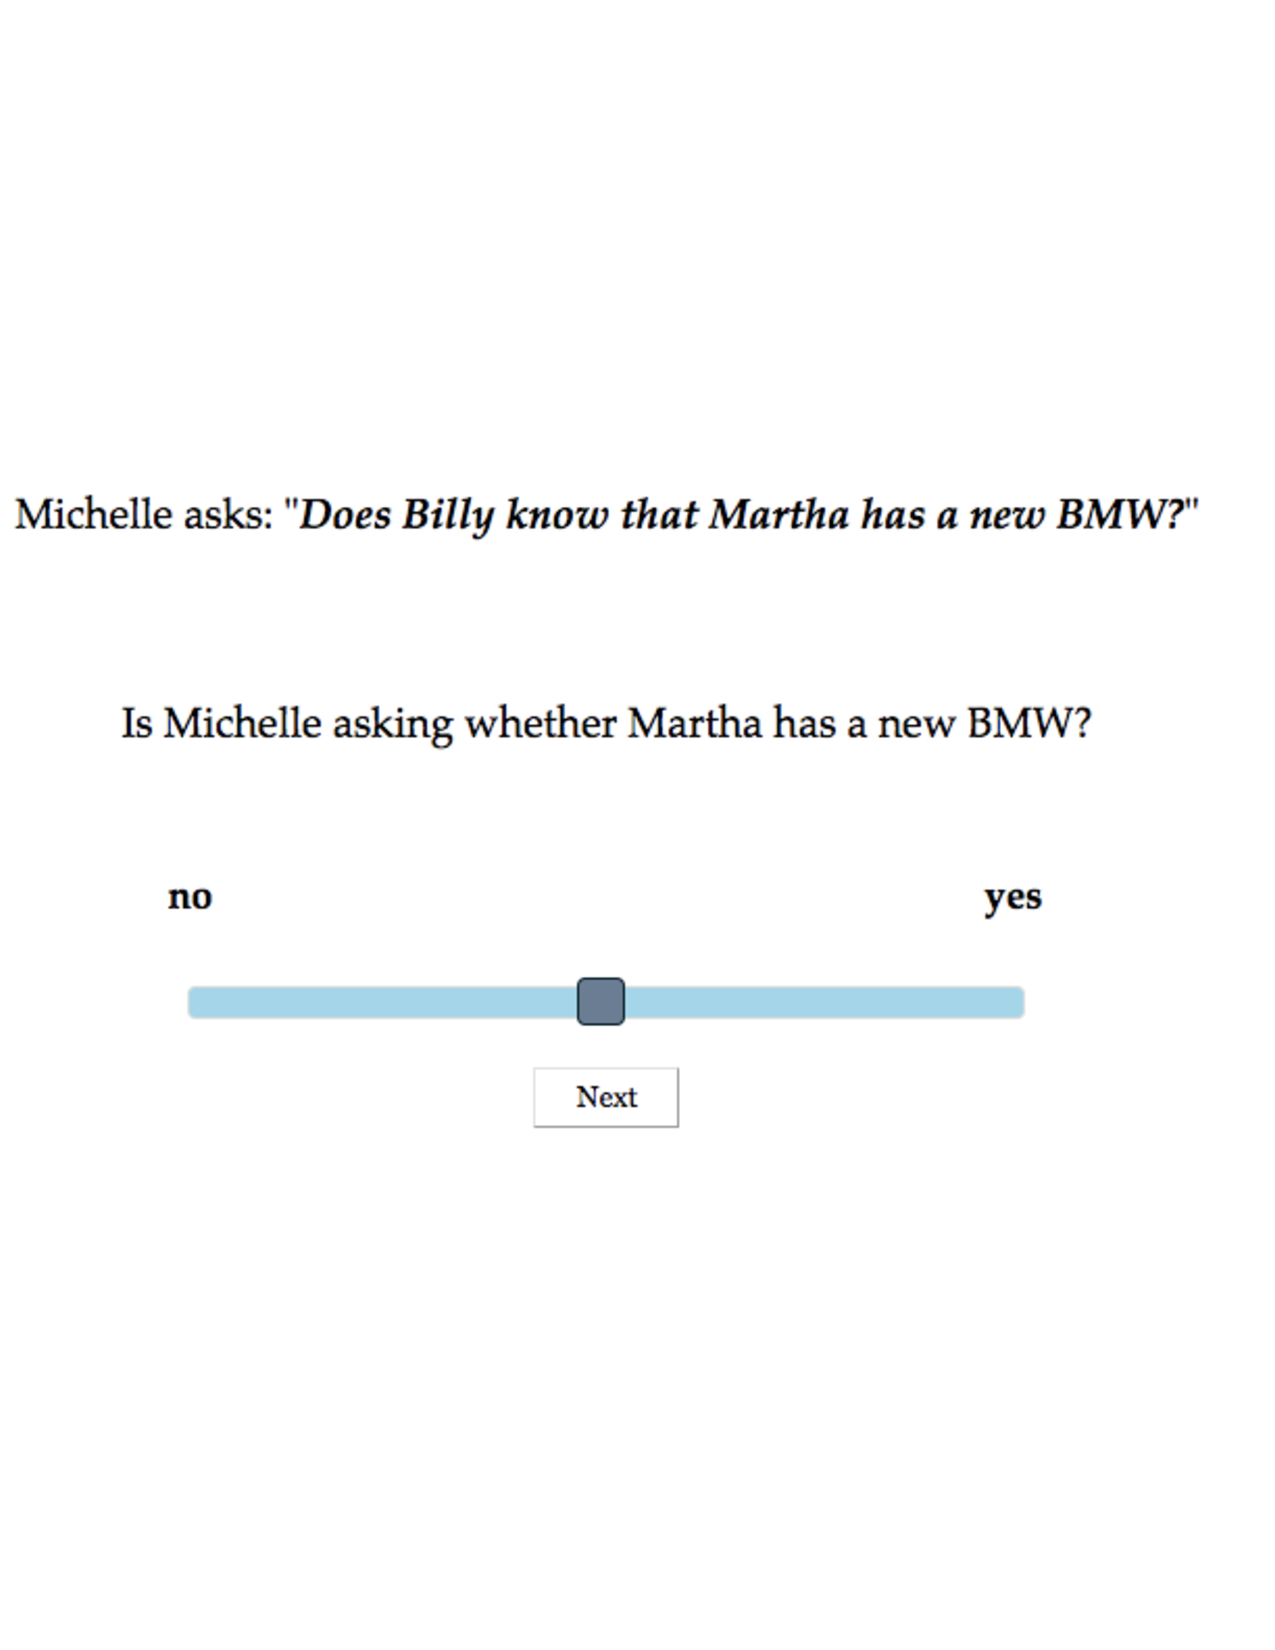
\includegraphics[width=12cm]{figures/exp1-trial}}
\end{center}
\caption{A sample (at-issueness) trial in Exp.~1}\label{f-trial-exp1}
\end{figure}

A `yes' response to a `certain that' question was taken to indicate that the person who uttered the polar question (e.g., Michelle in the sample trial) was committed to the relevant lexical content, i.e., that the lexical content projects, whereas a `no' response was taken to indicate that the lexical content did not project. For the `asking whether' questions, a `yes'  response was taken to indicate that the speaker was asking about the relevant lexical content, i.e., that it was at-issue, whereas a `no' response was taken to indicate that the lexical content was not at-issue. To explore the hypothesis that projectivity and not-at-issueness are positively related,  `yes' responses to `certain that' questions and `no' responses to `asking whether' questions were coded as 1; accordingly, `no' responses to `certain that' questions and `yes' responses to `asking whether' questions were coded as 0.

After completing the experiment, participants filled out a short optional survey about their age, their native language(s) and, if English is their native language, whether they are a speaker of American English (as opposed to, e.g., Australian or Indian English). To encourage them to respond truthfully, participants were told that they would be paid no matter what answers they gave in the survey.

\paragraph{Data exclusion.}
Prior to analysis, the data from 29 participants who did not self-identify as native speakers of American English were excluded. For the remaining 221 participants, we inspected their response means to the `certain that' and `asking whether' questions 
to the main clause controls: for these stimuli, we expect low responses to both types of questions since main clause contents are expected to be at-issue and not project. The response means of 11 participants were more than 3 standard deviations above the group means for at least one type of question (the group means were .07 for `certain that' and .04 for `asking whether' questions). Closer inspection revealed that these participants' responses to the control polar questions were systematically higher than the group means and involved 16 of the 17 lexical contents, suggesting that these participants did not attend to the task or interpreted the task differently. The data from these 11 participants were also excluded, leaving data from 210 participants (ages 19-68; median: 33).  


\subsubsection{Results}

We begin by addressing the two research questions in (\ref{questions}), namely whether there is projection variability across the projective contents of the target expressions and whether projectivity a function of at-issueness, as predicted by the Projection Principle. 

\paragraph{Projection variability across projective contents.} By-projective content variability can be seen in \figref{fig:proj-triggmeans}:  while median projectivity ratings were all close to ceiling (suggesting that for each projective content at least half of the participants took it to be robustly projective), the variable mean responses, box sizes and whisker lengths provide evidence of variability in projectivity across target expressions. For example, the mean projectivity of the prejacent of \emph{only} was relatively low at .76, while the mean projectivity of the projective contents of NRRCs and \emph{be annoyed} was close to ceiling at .96. \figref{fig:proj-subjmeans} shows that about one third of participants took the 9 projective contents they judged to be robustly projective. For the remaining participants, the decreasing means (from right to left) reveal a decrease in the overall projectivity of the 9 projective contents and the increasingly larger error bars reveal an increase in projection variability among the 9 projective contents. In sum, there is projection variability across the 9 projective contents.

\begin{figure}[h!]
\centering

\subfloat[][Boxplot of projection variability by expression, including main clause controls and collapsing across lexical contents. Grey dots indicate means and notches indicate medians. `MC' abbreviates main clause.]{ 
	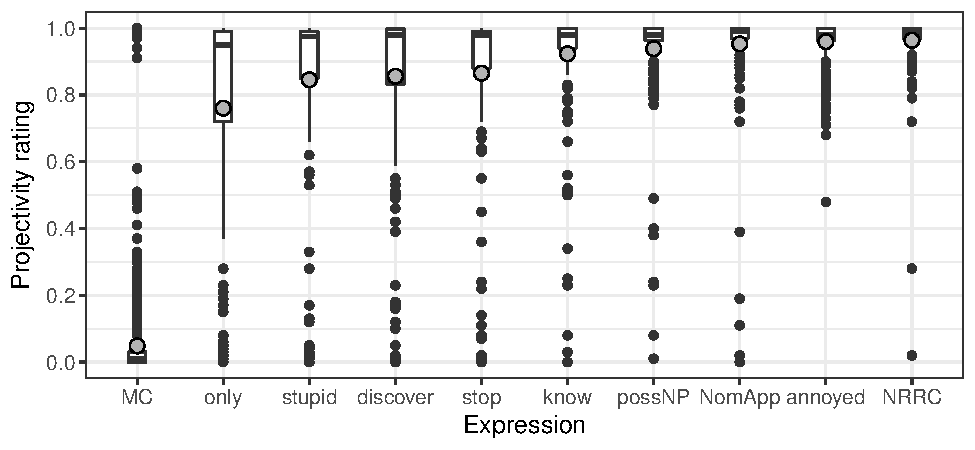
\includegraphics[width=12cm]{../results/exp1a/graphs/boxplot-projection-with-MCs}
	\label{fig:proj-triggmeans}
}

\subfloat[][Projectivity means by participant (excluding main clause controls). Error bars indicate bootstrapped 95\% confidence intervals.]{ 
	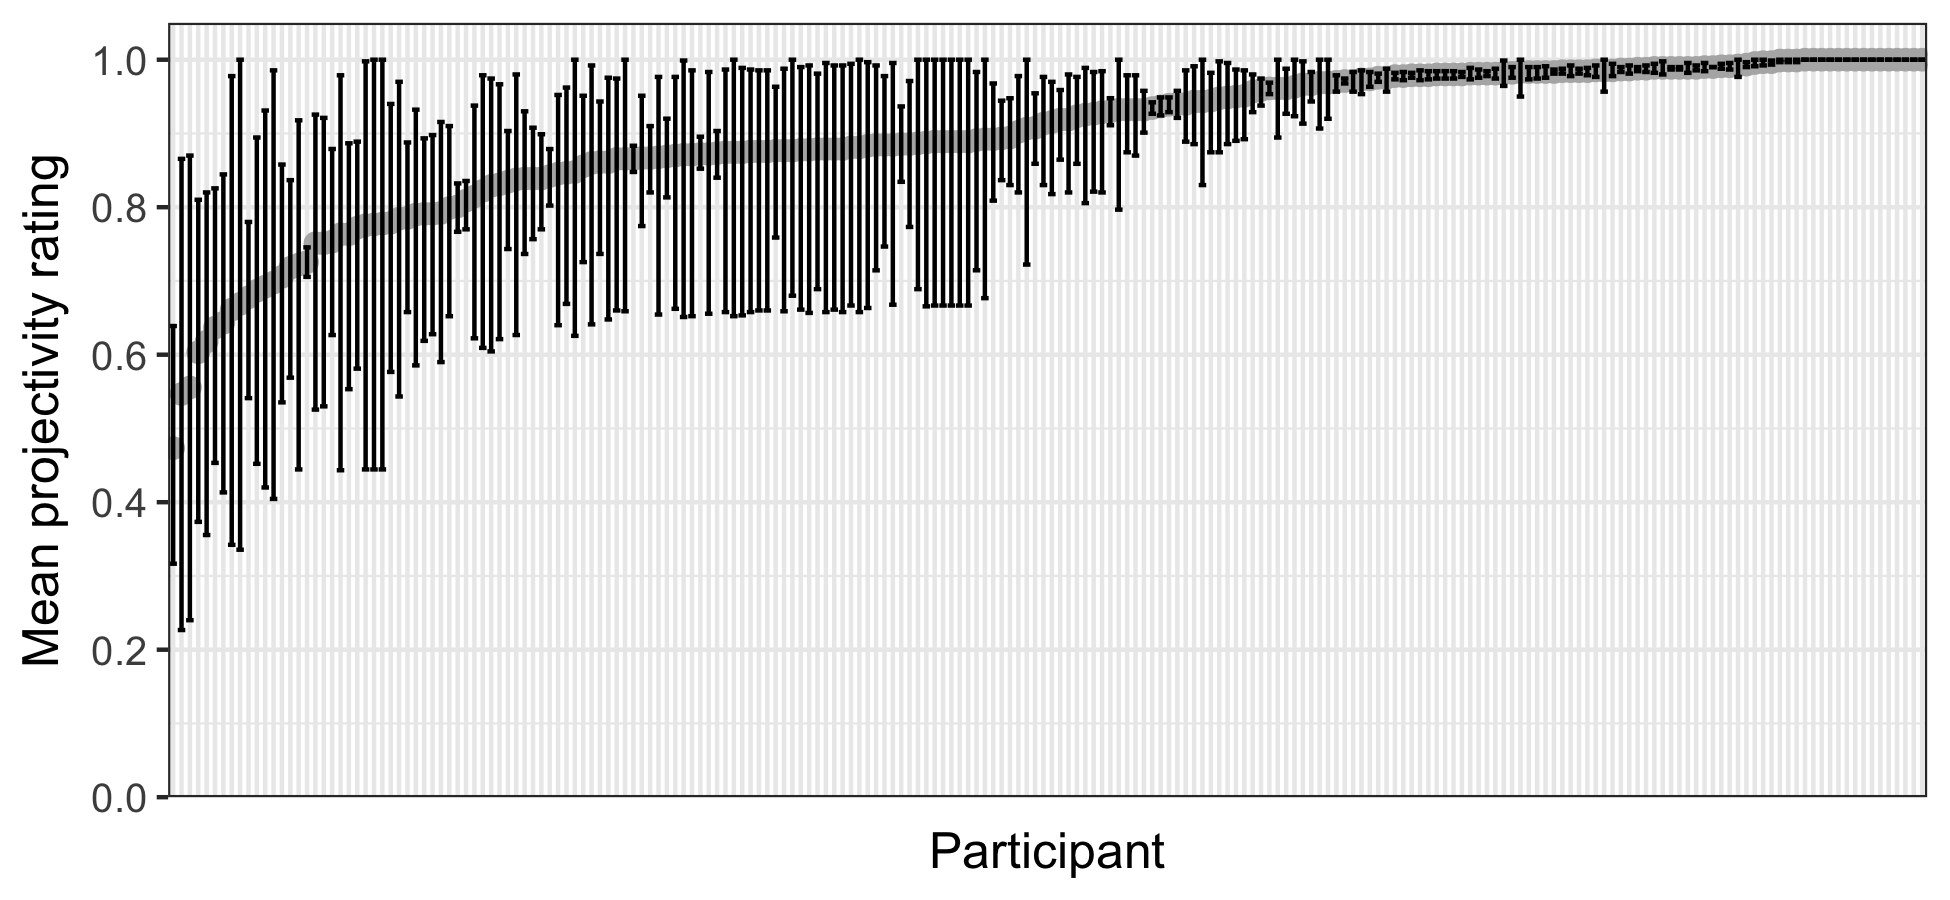
\includegraphics[width=12cm]{../results/exp1a/graphs/projection-subjectmeans}
	\label{fig:proj-subjmeans}
	}
	

\caption{Projectivity by expression (top panel) and by participant (bottom panel)}
\label{fig:f-proj-1a}
\end{figure}

To determine which projective contents differed from each other in projectivity, we conducted post hoc pairwise comparisons using Tukey's method (allowing for by-participant variability), using the \verb|lsmeans| package \citep{tukey} in R \citep{r}. P-values for each pair of target expression/projective content are displayed in \tableref{tab:pairwise}. These results suggest no difference in the projectivity of the projective contents of NRRCs, \emph{annoyed}, nominal appositives, possessive NPs, and \emph{know}. The projective contents of the other target expressions differed from each other in projectivity, except for the pairs \emph{discover/know} (which displayed only a marginally significant difference), \emph{discover/stop}, \emph{be stupid to/discover}, and \emph{be stupid to/stop}. 

%$lsmeans
% short_trigger    lsmean         SE      df  lower.CL  upper.CL
% annoyed       0.9595714 0.01473729 1675.74 0.9306660 0.9884769
% discover      0.8556667 0.01473729 1675.74 0.8267612 0.8845721
% know          0.9233810 0.01473729 1675.74 0.8944755 0.9522864
% NomApp        0.9528571 0.01473729 1675.74 0.9239517 0.9817626
% NRRC          0.9637619 0.01473729 1675.74 0.9348565 0.9926673
% only          0.7604286 0.01473729 1675.74 0.7315231 0.7893340
% possNP        0.9386667 0.01473729 1675.74 0.9097612 0.9675721
% stop          0.8650476 0.01473729 1675.74 0.8361422 0.8939531
% stupid        0.8455238 0.01473729 1675.74 0.8166184 0.8744293
%
%Degrees-of-freedom method: satterthwaite 
%Confidence level used: 0.95 
%
%$contrasts
% contrast               estimate         SE   df t.ratio p.value
% discover - annoyed -0.103904762 0.01947976 1680  -5.334  <.0001
% know - annoyed     -0.036190476 0.01947976 1680  -1.858  0.6431
% know - discover     0.067714286 0.01947976 1680   3.476  0.0153
% NomApp - annoyed   -0.006714286 0.01947976 1680  -0.345  1.0000
% NomApp - discover   0.097190476 0.01947976 1680   4.989  <.0001
% NomApp - know       0.029476190 0.01947976 1680   1.513  0.8496
% NRRC - annoyed      0.004190476 0.01947976 1680   0.215  1.0000
% NRRC - discover     0.108095238 0.01947976 1680   5.549  <.0001
% NRRC - know         0.040380952 0.01947976 1680   2.073  0.4923
% NRRC - NomApp       0.010904762 0.01947976 1680   0.560  0.9998
% only - annoyed     -0.199142857 0.01947976 1680 -10.223  <.0001
% only - discover    -0.095238095 0.01947976 1680  -4.889  <.0001
% only - know        -0.162952381 0.01947976 1680  -8.365  <.0001
% only - NomApp      -0.192428571 0.01947976 1680  -9.878  <.0001
% only - NRRC        -0.203333333 0.01947976 1680 -10.438  <.0001
% possNP - annoyed   -0.020904762 0.01947976 1680  -1.073  0.9780
% possNP - discover   0.083000000 0.01947976 1680   4.261  0.0007
% possNP - know       0.015285714 0.01947976 1680   0.785  0.9973
% possNP - NomApp    -0.014190476 0.01947976 1680  -0.728  0.9984
% possNP - NRRC      -0.025095238 0.01947976 1680  -1.288  0.9349
% possNP - only       0.178238095 0.01947976 1680   9.150  <.0001
% stop - annoyed     -0.094523810 0.01947976 1680  -4.852  <.0001
% stop - discover     0.009380952 0.01947976 1680   0.482  0.9999
% stop - know        -0.058333333 0.01947976 1680  -2.995  0.0689
% stop - NomApp      -0.087809524 0.01947976 1680  -4.508  0.0002
% stop - NRRC        -0.098714286 0.01947976 1680  -5.068  <.0001
% stop - only         0.104619048 0.01947976 1680   5.371  <.0001
% stop - possNP      -0.073619048 0.01947976 1680  -3.779  0.0051
% stupid - annoyed   -0.114047619 0.01947976 1680  -5.855  <.0001
% stupid - discover  -0.010142857 0.01947976 1680  -0.521  0.9999
% stupid - know      -0.077857143 0.01947976 1680  -3.997  0.0022
% stupid - NomApp    -0.107333333 0.01947976 1680  -5.510  <.0001
% stupid - NRRC      -0.118238095 0.01947976 1680  -6.070  <.0001
% stupid - only       0.085095238 0.01947976 1680   4.368  0.0005
% stupid - possNP    -0.093142857 0.01947976 1680  -4.782  0.0001
% stupid - stop      -0.019523810 0.01947976 1680  -1.002  0.9857
%
%P value adjustment: tukey method for comparing a family of 9 estimates  

\begin{table}[!h]
\begin{center}
\begin{tabular}{r c c c c c c c c}
\toprule
 &   NRRC & annoyed & NomApp &  possNP &  know & stop & discover & stupid \\
 \midrule
annoyed &  \emph{ns}  &  -  &        -   &       -  &        -  &   - &     -   &  -\\     
NomApp  &  \emph{ns} & \emph{ns} & -    &   -   &    -    &   -  &     -   & - \\    
possNP  &    \emph{ns} & \emph{ns} & \emph{ns} & - &      -  &     -     &  -   & - \\    
know     &   \emph{ns} & \emph{ns} & \emph{ns} & \emph{ns} & -   &    -   &    -       & -\\
stop     &   *** & *** & ** & ** & . & - &  - & -\\      
discover  &   *** & *** & *** & ** & * & \emph{ns} & - & -      \\
stupid    &  *** & *** & *** & *** & ** & \emph{ns} & \emph{ns} & - \\
only      &  *** & *** & *** & *** & *** & *** & *** & ** \\
\bottomrule
\end{tabular}
\caption{P-values associated with pairwise comparison of projective content projectivity means using Tukey's method. `***' indicates significance at .0001, `**' at .01, `*' at .05, `.' marginal significance at .1, and \emph{n.s} indicates no significant difference in means.}\label{tab:pairwise}
\end{center}
\end{table}

This brings us to our second research question: is projectivity a function of at-issueness, as predicted by the Projection Principle?

\paragraph{At-issueness.} Mean projectivity ratings for each target expression are visualized as a function of their mean not-at-issueness ratings in \figref{fig:f-proj-ai-1a} ($r =$ .85; when not collapsing across lexical contents $r =$ .45). There is a clear relationship between at-issueness and projectivity: projective contents that received higher projectivity ratings were also considered to be more not-at-issue.

\begin{figure}[!h]

\begin{center}
%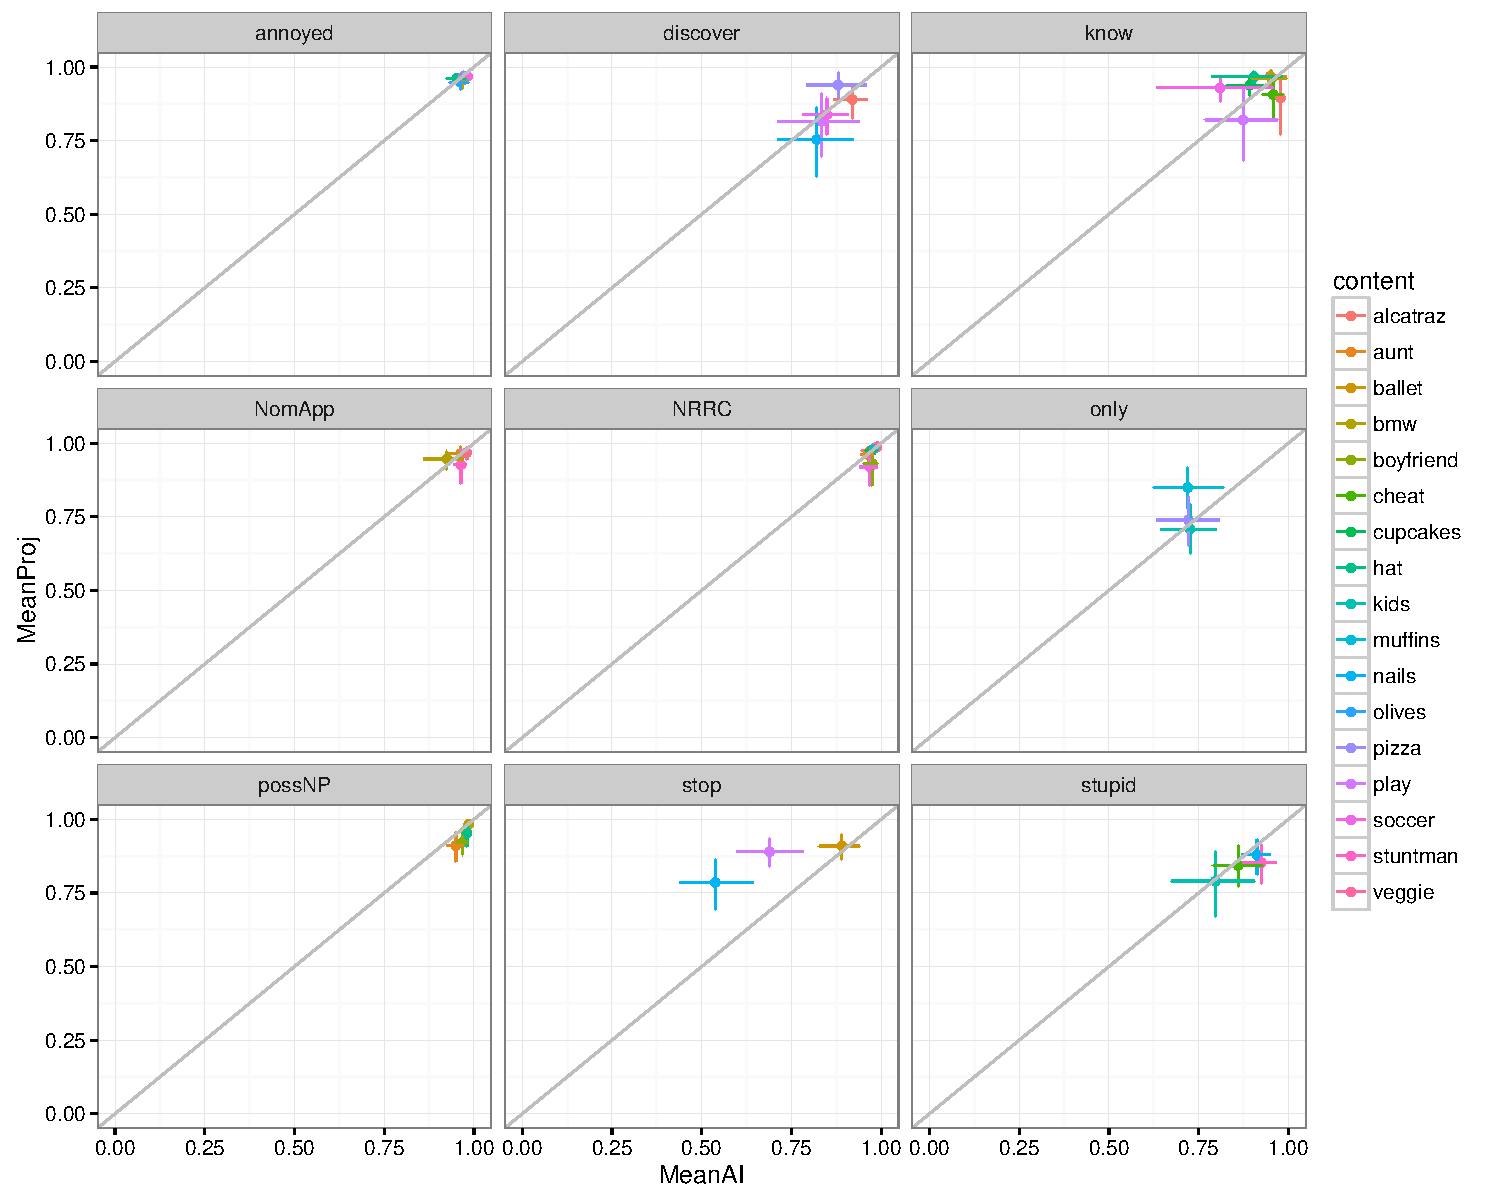
\includegraphics[width=12cm]{../results/exp1a/graphs/ai-proj-bytrigger}
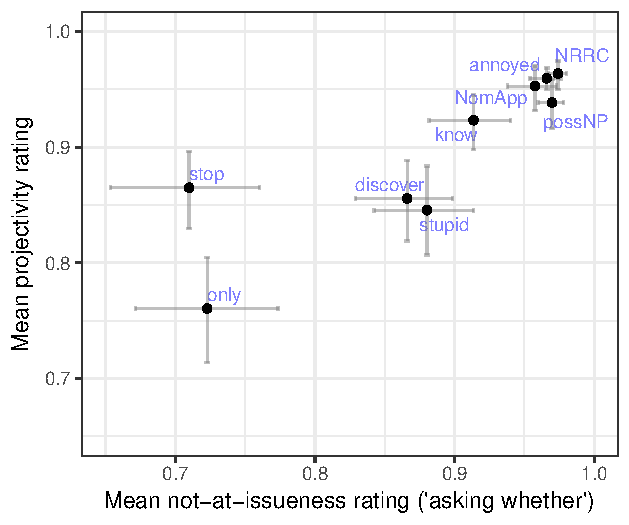
\includegraphics[width=10cm]{../results/exp1a/graphs/ai-proj-bytrigger-labels}
\end{center}

\caption{Mean projectivity against mean not-at-issueness by target expression/projective content. Error bars indicate bootstrapped 95\% confidence intervals. Dashed line indicates identical values on at-issueness and projectivity scales.}
\label{fig:f-proj-ai-1a}
\end{figure}

This qualitative observation about the relation between at-issueness and projectivity was borne out statistically. We conducted a mixed-effects linear regression predicting projectivity rating from a centered fixed effect of at-issueness rating. In order to control for block order effects, the model also included a centered fixed effect of block order and the interaction of block order and at-issueness. The model included the maximal random effects structure justified by the data and the theoretical assumptions: random by-expression intercepts (capturing differences in projectivity between target expressions),  random by-lexical content intercepts (capturing differences in projectivity between lexical contents), random by-participant intercepts (capturing individual variability in projectivity) and random slopes for at-issueness by target expression, lexical content, and participant (capturing that the effect of at-issueness may vary across target expressions, lexical contents, and participants). Here and in the remainder of the paper, p-values were obtained by likelihood ratio tests of the full model with the effect in question against the model without the effect in question. The analysis was conducted on non-main-clause trials only (1,890 data points) because we were specifically interested in variability in projectivity for contents that have the potential to project. Analyses were conducted using the \verb|lme4| package \citep{bates2015}.

There was a significant main effect of at-issueness such that more not-at-issue items received higher projectivity ratings ($\beta$ = 0.37, $SE$ = 0.10, $t$ = 3.70, $\chi^2(1)$ = 9.20, $p <$ .003). This finding suggests that projectivity a function of at-issueness, i.e., the information-structural status of projective content, as predicted by the Projection Principle. Likelihood ratio tests revealed that each random effect was justified (see \tableref{tab:random1a} for standard deviations and p-values); that is, there was by-participant, by-expression and by-lexical content variability in projectivity, as well as variability in the at-issueness effect across participants, target expressions and lexical contents. Thus, in addition to at-issueness, the projectivity of the projective content was also influenced by the participant who gave the rating, the expression associated with the projective content and the lexical content that instantiated the projective content. The block effect did not reach significance ($\beta$ = -0.02, $SE$ = 0.01, $t$ = -1.56, $\chi^2(1)$ = 2.39, $p >$ .12), nor did the interaction term ($\beta$ = 0.08, $SE$ = 0.08, $t$ = 0.98, $\chi^2(1)$ = 0.96, $p >$ .32), suggesting that the order in which participants completed the tasks (projectivity, at-issueness) did not affect their judgments in a systematic way. 

% Random effects:
% Groups        Name        Variance Std.Dev. Corr 
% workerid      (Intercept) 0.003534 0.05945       
%               cai         0.152839 0.39095  -0.69
% content       (Intercept) 0.000613 0.02476       
%               cai         0.034367 0.18538  -0.74
% short_trigger (Intercept) 0.001353 0.03678       
%               cai         0.048460 0.22014  -0.73
% Residual                  0.025980 0.16118       
%Number of obs: 1890, groups:

\begin{table}
\begin{tabular}{c c c c c c }
\toprule
\multicolumn{3}{c}{Intercepts} & \multicolumn{3}{c}{Slopes for at-issueness}\\
Target expression & Lexical content & Participant & Target expression & Lexical content & Participant\\
\midrule
.04 & .02 & .06 & .22 & .19 & .39\\
$< .0001$ & $< .003$ & $< .0001$ & $< .0001$ & $< .0001$ & $< .0001$ \\
\bottomrule
\end{tabular}
\caption{Standard deviations (first row) and p-values (second row, $\chi^2(2)$) for random effects in Exp.~1a model.}\label{tab:random1a}
\end{table}

%
%\begin{figure}[!h]
%\begin{center}
%
%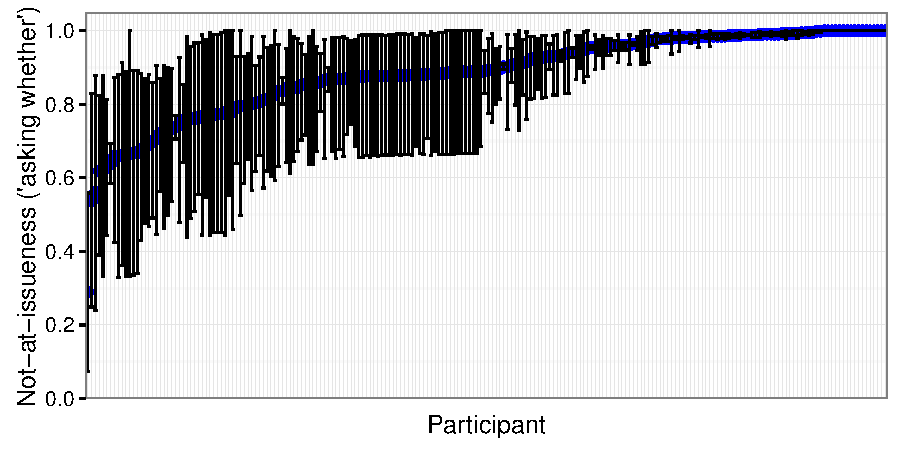
\includegraphics[width=12cm]{../results/exp1a/graphs/ai-subjectmeans}
%
%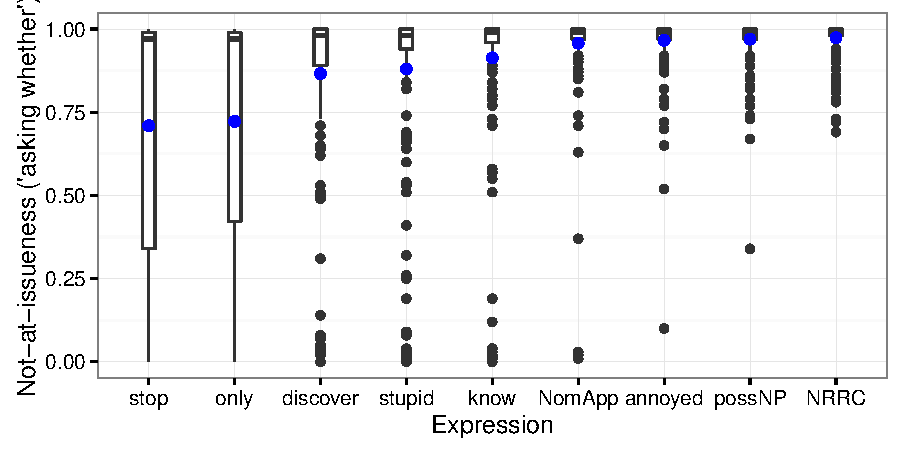
\includegraphics[width=12cm]{../results/exp1a/graphs/boxplot-not-at-issueness}
%
%\end{center}
%\caption{At-issueness by participant (top panel) and projective content trigger (bottom panel) \jd{not sure this is an interesting plot}}
%\label{f-ai-1a}
%\end{figure}
%
%


\subsubsection{Discussion}\label{s-discussion1a}

Exp.~1a was designed to explore projection variability for projective contents associated with a set of syntactically heterogeneous target expressions and to test the Projection Principle, which holds that the projectivity of projective content is related to its information-structural status. The experiment provided robust empirical evidence for projection variability across the 9 projective contents. Furthermore, the experiment provided evidence for projection variability across participants. This finding suggests that speakers of American English differ in the extent to which they take the projective contents associated with the 9 target expressions to project. Finally, the experiment also showed that the lexical content that instantiates a projective content plays a role in the extent to which the projective content projects. A methodological implication of these latter two findings is that research on projective content must be sensitive to potential inter-speaker and inter-lexical content differences.

The experiment also provided empirical support for the Projection Principle since the at-issueness of projective content was a significant predictor of its projectivity. This finding suggests that the extent to which a speaker is taken to be committed to a particular projective content is related to the extent to which the projective content is at-issue in the speaker's utterance. The experiment also showed that the target expressions differ in the extent to which the projective content they are associated with projects. This finding suggests that both the information-structural status of the projective content and the conventional meaning of the target expressions may play a role the extent to which a speaker is taken to be committed to a projective content. We discuss implications of these findings in sections \ref{s-summary1a1b} and \ref{s5}, after presenting the findings of Exps.~1b and 2.

\subsection{Experiment 1b}\label{s-exp1b} 

Exp.~1b was designed to explore the projectivity and at-issueness of the projective contents of the 12 syntactically more homogeneous predicates in (\ref{pairs1b2b}), i.e., the contents of the complements of the emotive `factives' {\em be amused} and {\em be annoyed}, the cognitive `factive' {\em be aware}, the sensory `factive' {\em see}, the cognitive `semi-factives' {\em discover, find out, notice, realize, learn} and {\em establish}, and the communication `semi-factives' {\em confess} and {\em reveal}.


\subsubsection{Methods}

\paragraph{Participants.} 250 participants with U.S.\ IP addresses and at least 97\% of previous HITs approved were recruited on Amazon's Mechanical Turk platform (ages: 18-74; median: 32). They were paid \$1 for participating in the experiment.

\paragraph{Materials.} The 12 projective contents explored in this experiment were instantiated by 20 lexical contents, which are given in Appendix \ref{a-lexcontents1b}.  Each of the 12 projective contents was instantiated by each of these 20 lexical contents, for a total of 240 target stimuli. The target stimuli were (past and present tense)\footnote{The main clauses of stimuli with {\em be amused, be aware} and {\em be annoyed} were realized in the present tense; the main clauses of stimuli with the other predicates were realized in the past tense.} polar questions formed from sentences with one of the 12 predicates, a clausal complement formed from one of the 20 lexical contents and a random proper name subject (the names used for the subjects did not occur in the clausal complements or as the speakers). Two sample target stimuli are given in (\ref{sample2}): the complement clause in both stimuli is instantiated by the lexical content `Raul was drinking chamomile tea'.

\begin{exe}
\ex\label{sample2}
\begin{xlist}
\ex Emily asks: Is Shirley aware that Raul was drinking chamomile tea?

\ex Gary asks: Did Samuel discover that Raul was drinking chamomile tea?
\end{xlist}
\end{exe}

The experiment also included 20 control stimuli, which were (past tense) polar questions formed from sentences conveying the 20 lexical contents; a sample control polar question formed is shown in (\ref{sample3}). The control stimuli were included to confront participants with contents that are at-issue and not projective, and to assess whether participants were attending to the task.

\begin{exe}
\ex\label{sample3} Timothy asks: Was Raul drinking chamomile tea?
\end{exe}

For each participant, a set of 20 polar question stimuli was randomly created: each set contained a target polar question for each of the 12 target expressions (the projective content associated with each expression was instantiated by a unique lexical content) and 8 control polar questions (with unique lexical contents as well, for a total of 20 unique lexical contents). Each participants saw their 20 polar question stimuli twice, for a total of 40 trials: in one block, participants responded to `certain that' questions to assess projectivity; in the other block, participants responded to `asking whether' questions to assess at-issueness. Block order and within-block trial order were randomized.

\paragraph{Procedure.} The procedure of Exp.~1b was the same as for Exp.~1a, described in section \ref{s-methods-1a}, except that participants responded to 20 `certain that' and 20 `asking whether' questions. (There are more trials in Exp.~1b than in Exp.~1a because each participant judged the projectivity and at-issueness of 20  rather than 15 contents.)


\paragraph{Data exclusion.} Prior to analysis, we excluded the data from 3 participants who did not self-identify as native speakers of American English. For the remaining 247 participants, we inspected their response means to the `certain that' and `asking whether' questions to the main clause controls. The response means of 12 participants were more than 3 standard deviations above the group means for at least one type of question (the group means were .08 for `certain that' and .04 for `asking whether' questions). Further inspection revealed that these participants' responses to the control questions were systematically higher than the group means and involved all of the 20 lexical contents, suggesting that these participants did not attend to the task or interpreted the task differently. The data from these 12 participants were also excluded, leaving data from 235 participants (ages 18-74; median: 33).

\subsubsection{Results}

\paragraph{Projection variability across projective contents.} We begin by addressing the research question in (\ref{questions}a), whether the projective contents associated with the 12 target expressions exhibit projection variability. Variability in how robustly the contents of the clausal complements of the 12 (semi-)factive predicates project can be seen in \figref{fig:proj-triggmeans-1b}. The median projectivity ratings are at ceiling for the contents of the clausal complements of most of the (semi-)factive predicates, suggesting that at least half of the participants took these contents to be robustly projective. The exceptions are the predicates {\em established, confessed} and {\em revealed}, for which the medians are not at ceiling, suggesting that the speaker was less likely to be taken to be committed to the contents of the complements of these predicates than for the other 9 predicates. Variability in how robustly the contents of the clausal complements of the 12 predicates is also suggested by variable mean responses, box sizes and whisker lengths across the projective contents of the 12 predicates. \figref{fig:proj-subjmeans-1b} shows that relatively few participants took the contents of the complements of all 12 predicates to be robustly projective. The mean responses suggest that there is by-participant variability in how robustly the contents of the complements of the 12 predicates were taken to project.

\begin{figure}[!h]
\centering

\subfloat[][Boxplot of projection variability by expression, including main clause controls and collapsing across lexical contents. Grey dots indicate means and notches indicate medians. `MC' abbreviates main clause.]{ 
	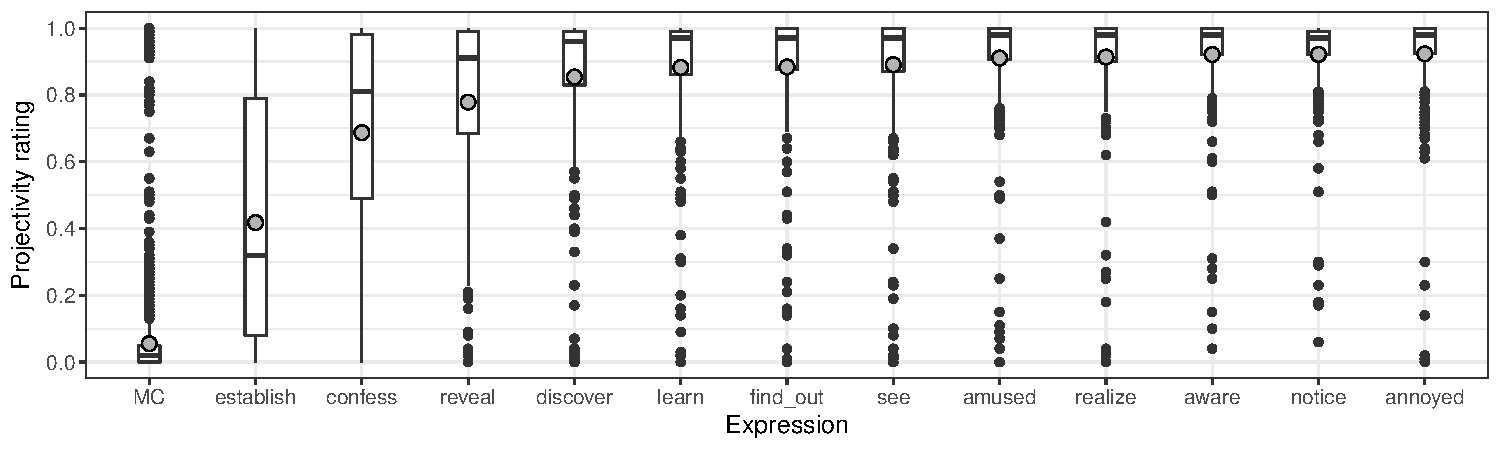
\includegraphics[width=16cm]{../results/exp1b/graphs/boxplot-projection-with-MCs}
	\label{fig:proj-triggmeans-1b}
}

\subfloat[][Projectivity means by participant (excluding main clause controls). Error bars indicate bootstrapped 95\% confidence intervals.]{ 
	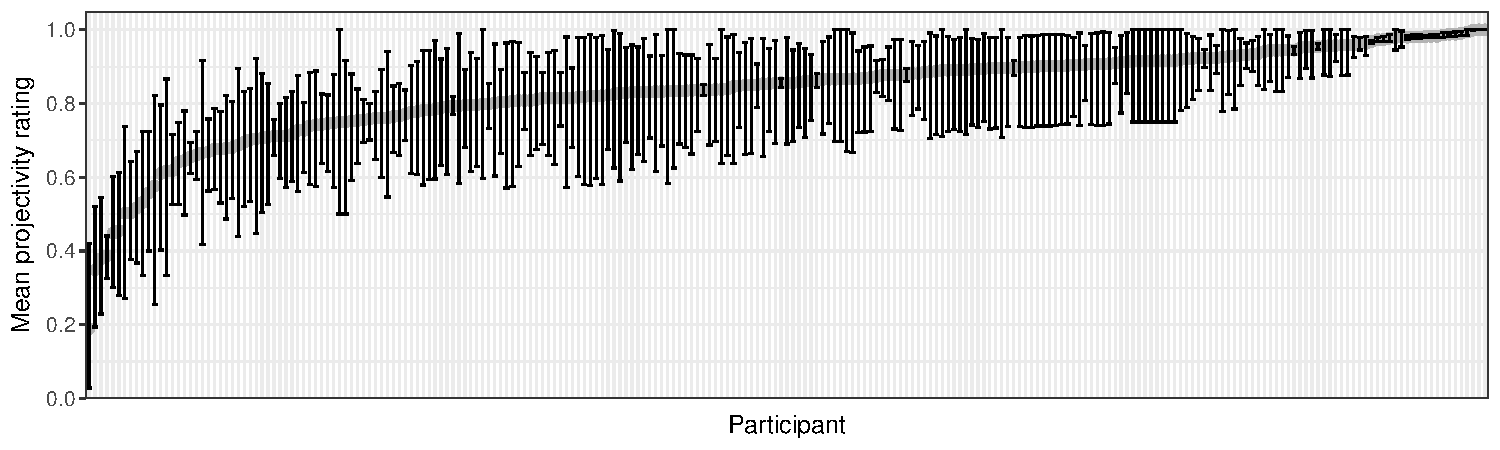
\includegraphics[width=16cm]{../results/exp1b/graphs/projection-subjectmeans}
	\label{fig:proj-subjmeans-1b}
	}
	
\caption{Projectivity by expression (top panel) and by participant (bottom panel)}\label{fig:f-proj-1b}
\end{figure}

As in Exp.~1a,  we conducted post hoc pairwise comparisons using Tukey's method to determine which of the projective contents associated with the 12 target expressions differed from each other in projectivity. P-values for each pair of target expression/projective content are displayed in \tableref{tab:pairwise-1b}. The results suggest no difference in the projectivity of the projective contents of \emph{be annoyed}, \emph{notice}, \emph{be aware}, \emph{realize}, \emph{be amused}, \emph{see}, and \emph{find out}. The projective contents of the other predicates differed from each other in projectivity, with the exception of the pairs \emph{discover/see}, \emph{discover/find out}, and \emph{discover/learn}. Furthermore, \emph{discover} was  marginally different from \emph{be aware}, \emph{realize}, and \emph{be amused}).

%$lsmeans
% short_trigger    lsmean         SE     df  lower.CL  upper.CL
% confessed     0.6869787 0.01499147 1739.4 0.6575755 0.7163819
% discovered    0.8534043 0.01499147 1739.4 0.8240011 0.8828075
% established   0.4177447 0.01499147 1739.4 0.3883415 0.4471479
% found_out     0.8837447 0.01499147 1739.4 0.8543415 0.9131479
% is_amused     0.9102979 0.01499147 1739.4 0.8808947 0.9397011
% is_annoyed    0.9228936 0.01499147 1739.4 0.8934904 0.9522968
% is_aware      0.9208936 0.01499147 1739.4 0.8914904 0.9502968
% learned       0.8821277 0.01499147 1739.4 0.8527245 0.9115309
% noticed       0.9212340 0.01499147 1739.4 0.8918308 0.9506372
% realize       0.9133191 0.01499147 1739.4 0.8839159 0.9427224
% revealed      0.7784255 0.01499147 1739.4 0.7490223 0.8078287
% saw           0.8905957 0.01499147 1739.4 0.8611925 0.9199989
%
%Degrees-of-freedom method: satterthwaite 
%Confidence level used: 0.95 
%
%$contrasts
% contrast                      estimate         SE   df t.ratio p.value
% discovered - confessed    0.1664255319 0.01851128 2585   8.990  <.0001
% established - confessed  -0.2692340426 0.01851128 2585 -14.544  <.0001
% established - discovered -0.4356595745 0.01851128 2585 -23.535  <.0001
% found_out - confessed     0.1967659574 0.01851128 2585  10.630  <.0001
% found_out - discovered    0.0303404255 0.01851128 2585   1.639  0.8946
% found_out - established   0.4660000000 0.01851128 2585  25.174  <.0001
% is_amused - confessed     0.2233191489 0.01851128 2585  12.064  <.0001
% is_amused - discovered    0.0568936170 0.01851128 2585   3.073  0.0892
% is_amused - established   0.4925531915 0.01851128 2585  26.608  <.0001
% is_amused - found_out     0.0265531915 0.01851128 2585   1.434  0.9568
% is_annoyed - confessed    0.2359148936 0.01851128 2585  12.744  <.0001
% is_annoyed - discovered   0.0694893617 0.01851128 2585   3.754  0.0097
% is_annoyed - established  0.5051489362 0.01851128 2585  27.289  <.0001
% is_annoyed - found_out    0.0391489362 0.01851128 2585   2.115  0.6121
% is_annoyed - is_amused    0.0125957447 0.01851128 2585   0.680  0.9999
% is_aware - confessed      0.2339148936 0.01851128 2585  12.636  <.0001
% is_aware - discovered     0.0674893617 0.01851128 2585   3.646  0.0144
% is_aware - established    0.5031489362 0.01851128 2585  27.181  <.0001
% is_aware - found_out      0.0371489362 0.01851128 2585   2.007  0.6889
% is_aware - is_amused      0.0105957447 0.01851128 2585   0.572  1.0000
% is_aware - is_annoyed    -0.0020000000 0.01851128 2585  -0.108  1.0000
% learned - confessed       0.1951489362 0.01851128 2585  10.542  <.0001
% learned - discovered      0.0287234043 0.01851128 2585   1.552  0.9258
% learned - established     0.4643829787 0.01851128 2585  25.086  <.0001
% learned - found_out      -0.0016170213 0.01851128 2585  -0.087  1.0000
% learned - is_amused      -0.0281702128 0.01851128 2585  -1.522  0.9348
% learned - is_annoyed     -0.0407659574 0.01851128 2585  -2.202  0.5481
% learned - is_aware       -0.0387659574 0.01851128 2585  -2.094  0.6271
% noticed - confessed       0.2342553191 0.01851128 2585  12.655  <.0001
% noticed - discovered      0.0678297872 0.01851128 2585   3.664  0.0135
% noticed - established     0.5034893617 0.01851128 2585  27.199  <.0001
% noticed - found_out       0.0374893617 0.01851128 2585   2.025  0.6761
% noticed - is_amused       0.0109361702 0.01851128 2585   0.591  1.0000
% noticed - is_annoyed     -0.0016595745 0.01851128 2585  -0.090  1.0000
% noticed - is_aware        0.0003404255 0.01851128 2585   0.018  1.0000
% noticed - learned         0.0391063830 0.01851128 2585   2.113  0.6138
% realize - confessed       0.2263404255 0.01851128 2585  12.227  <.0001
% realize - discovered      0.0599148936 0.01851128 2585   3.237  0.0555
% realize - established     0.4955744681 0.01851128 2585  26.771  <.0001
% realize - found_out       0.0295744681 0.01851128 2585   1.598  0.9102
% realize - is_amused       0.0030212766 0.01851128 2585   0.163  1.0000
% realize - is_annoyed     -0.0095744681 0.01851128 2585  -0.517  1.0000
% realize - is_aware       -0.0075744681 0.01851128 2585  -0.409  1.0000
% realize - learned         0.0311914894 0.01851128 2585   1.685  0.8753
% realize - noticed        -0.0079148936 0.01851128 2585  -0.428  1.0000
% revealed - confessed      0.0914468085 0.01851128 2585   4.940  0.0001
% revealed - discovered    -0.0749787234 0.01851128 2585  -4.050  0.0031
% revealed - established    0.3606808511 0.01851128 2585  19.484  <.0001
% revealed - found_out     -0.1053191489 0.01851128 2585  -5.689  <.0001
% revealed - is_amused     -0.1318723404 0.01851128 2585  -7.124  <.0001
% revealed - is_annoyed    -0.1444680851 0.01851128 2585  -7.804  <.0001
% revealed - is_aware      -0.1424680851 0.01851128 2585  -7.696  <.0001
% revealed - learned       -0.1037021277 0.01851128 2585  -5.602  <.0001
% revealed - noticed       -0.1428085106 0.01851128 2585  -7.715  <.0001
% revealed - realize       -0.1348936170 0.01851128 2585  -7.287  <.0001
% saw - confessed           0.2036170213 0.01851128 2585  11.000  <.0001
% saw - discovered          0.0371914894 0.01851128 2585   2.009  0.6873
% saw - established         0.4728510638 0.01851128 2585  25.544  <.0001
% saw - found_out           0.0068510638 0.01851128 2585   0.370  1.0000
% saw - is_amused          -0.0197021277 0.01851128 2585  -1.064  0.9960
% saw - is_annoyed         -0.0322978723 0.01851128 2585  -1.745  0.8472
% saw - is_aware           -0.0302978723 0.01851128 2585  -1.637  0.8955
% saw - learned             0.0084680851 0.01851128 2585   0.457  1.0000
% saw - noticed            -0.0306382979 0.01851128 2585  -1.655  0.8881
% saw - realize            -0.0227234043 0.01851128 2585  -1.228  0.9868
% saw - revealed            0.1121702128 0.01851128 2585   6.060  <.0001
%
%P value adjustment: tukey method for comparing a family of 12 estimates


\begin{table}[!h]
\begin{center}
\begin{tabular}{l l l l l l l l l l l l }
\toprule
 &   \rot{be annoyed} & \rot{notice} & \rot{be aware} &  \rot{realize} &  \rot{be amused} & \rot{see} & \rot{find out} & \rot{learn} & \rot{discover} & \rot{reveal} & \rot{confess} \\
 \midrule
notice & \emph{n.s} & - & - & - & - & - & - & - & - & - & - \\ 
be aware & \emph{n.s} & \emph{n.s} & -&- &- &- &- &- &- &- &-  \\ 
realize & \emph{n.s} & \emph{n.s} & \emph{n.s} & - & - &- &- &- &- &- &-  \\ 
be amused & \emph{n.s} & \emph{n.s} & \emph{n.s} & \emph{n.s} & - & - & - & - & - & - & -  \\ 
see & \emph{n.s} & \emph{n.s} & \emph{n.s} & \emph{n.s} & \emph{n.s} & - &- &- &- &- &-  \\ 
find out & \emph{n.s} & \emph{n.s} & \emph{n.s} & \emph{n.s} & \emph{n.s}& \emph{n.s} & -& -& -& -& -\\ 
learn  & \emph{n.s} & \emph{n.s} & \emph{n.s} & \emph{n.s} & \emph{n.s} & \emph{n.s} & \emph{n.s}  & - & - & - & - \\ 
discover & ** & * & . & . & . & \emph{n.s} & \emph{n.s} & \emph{n.s.} & - &- &-  \\ 
reveal  & *** & ***  & *** & *** & *** & *** & *** & *** & ** & -&-  \\   
confess  & *** & *** & *** & *** & *** & *** & *** &  *** & *** & *** & - \\ 
establish    & *** & *** & *** & *** & *** & *** & *** & *** & *** & *** & *** \\
\bottomrule
\end{tabular}

\caption{P-values associated with pairwise comparison of projective contents associated with target expressions using Tukey's method. `***' indicates significance at .0001, `**' at .01, `*' at .05, `.' marginal significance at .1, and \emph{n.s} indicates no significant difference in means.}\label{tab:pairwise-1b}
\end{center}

\end{table}


As for the observed variability in Exp.~1a, we now ask: is projectivity a function of at-issueness, as predicted by the Projection Principle?

\paragraph{At-issueness.} Mean projectivity ratings for the projective content associated with each target expression are visualized in \figref{fig:f-proj-ai-1b} as a function of their mean not-at-issueness ratings ($r =$ .82; when not collapsing across lexical contents $r =$ .44). There is a clear relationship between at-issueness and projectivity: projective contents that received higher not-at-issueness ratings were considered to be more projective.

\begin{figure}[!h]

\begin{center}
%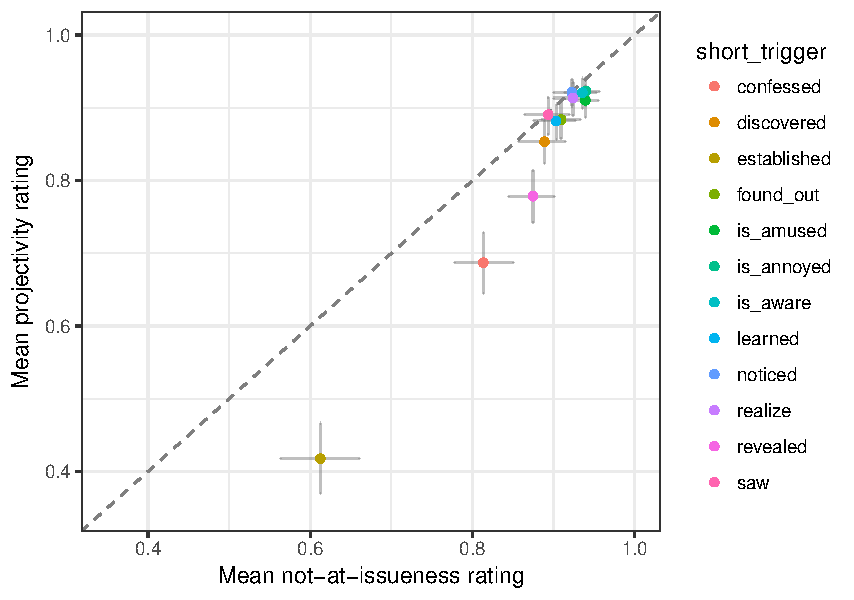
\includegraphics[width=12cm]{../results/exp1b/graphs/ai-proj-bytrigger}
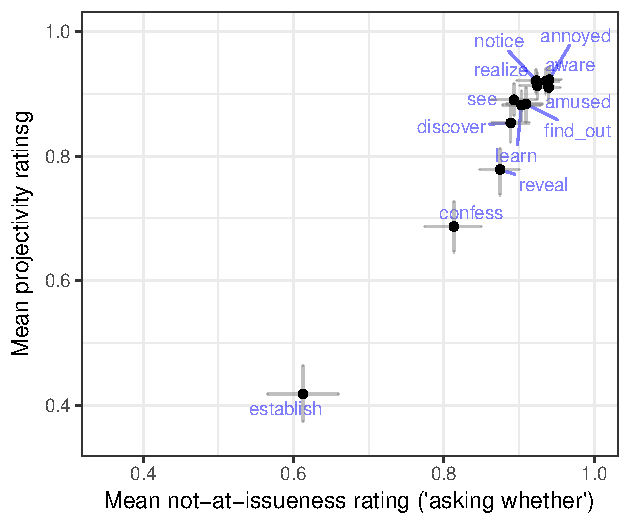
\includegraphics[width=10cm]{../results/exp1b/graphs/ai-proj-bytrigger-labels}
\end{center}

\caption{Mean projectivity against mean not-at-issueness by target expression. Error bars indicate bootstrapped 95\% confidence intervals. Dashed line indicates identical values on at-issueness and projectivity scales.}
\label{fig:f-proj-ai-1b}
\end{figure}

This qualitative observation about the relation between at-issueness and projectivity was again borne out statistically. We conducted an appropriately adjusted variant of the mixed-effects linear regression analysis of Exp.~1a. The model predicted projectivity rating from centered fixed effects of at-issueness rating, block order, and the interaction of block order and at-issueness. The model included the maximal random effects structure that allowed the model to converge: random by-expression intercepts (capturing differences in projectivity between target expressions),  random by-participant intercepts (capturing individual variability in projectivity), and random slopes for at-issueness by target expression, lexical content, and participant (capturing that the effect of at-issueness may vary across target expressions, lexical contents, and participants). In contrast to the model reported in the previous section, the current model did not contain random by-lexical content intercepts because there was no by-lexical content intercept variability. As before, the analysis was conducted on non-main-clause trials only (2,820 data points).

We observed a significant main effect of at-issueness, such that more not-at-issue items received higher projectivity ratings ($\beta$ = 0.34, $SE$ = 0.04, $t$ = 9.31, $\chi^2(1)$ = 31.36, $p <$ .0001). This finding suggests again that the information-structural status of a projective content is related to its projectivity, as predicted by the Projection Principle. Likelihood ratio tests revealed that of the included random effects, by-lexical content and by-expression slopes for at-issueness were not justified (see \tableref{tab:random1b} for standard deviations and p-values); that is, there was by-participant and by-expression variability in projectivity, as well as variability in the at-issueness effect across participants, but in contrast to the data collected in Exp.~1a, there was no variability in the at-issueness effect across target expressions and lexical contents. Together, these findings suggest again that there are target expression-specific effects in projectivity, but overall less random variability, especially across lexical contents. 

The block effect did not reach significance ($\beta$ = -0.02, $SE$ = 0.01, $t$ = -1.43, $\chi^2(1)$ = 2.02, $p >$ .15), but the interaction term did ($\beta$ = 0.21, $SE$ = 0.05, $t$ = 3.83, $\chi^2(1)$ = 14.09, $p <$ .0002). Simple effects analysis revealed that this was due to a difference in slope: while there was an effect of at-issueness on projectivity in the predicted direction regardless of block order, the effect was greater in the group of participants who performed the projectivity task first ($\beta$ = 0.44, $SE$ = 0.05, $t$ = 9.33) than in the group who performed the at-issueness task first ($\beta$ = 0.24, $SE$ = 0.04, $t$ = 5.46).

%Random effects:
% Groups        Name        Variance Std.Dev. Corr 
% workerid      (Intercept) 0.008759 0.09359       
%               cai         0.054466 0.23338  -0.29
% content       cai         0.001486 0.03855       
% short_trigger (Intercept) 0.013314 0.11539       
%               cai         0.003151 0.05613  0.30 
% Residual                  0.035808 0.18923       
%Number of obs: 2820, groups:  

\begin{table}
\begin{center}
\begin{tabular}{c c c c c c }
\toprule
\multicolumn{2}{c}{Intercepts} & \multicolumn{3}{c}{Slopes for at-issueness}\\
Target expression & Participant & Target expression & Lexical content & Participant\\
\midrule
.12 & .09 & .06 & .04 & .23\\
$< .0001$ & $< .0001$ & $> .20$ & $> .50$ & $< .0001$ \\
\bottomrule
\end{tabular}
\caption{Standard deviations (first row) and p-values (second row, $\chi^2(2)$) for random effects in Exp.~1b model.}\label{tab:random1b}
\end{center}
\end{table}

%
%\begin{figure}[!h]
%\begin{center}
%
%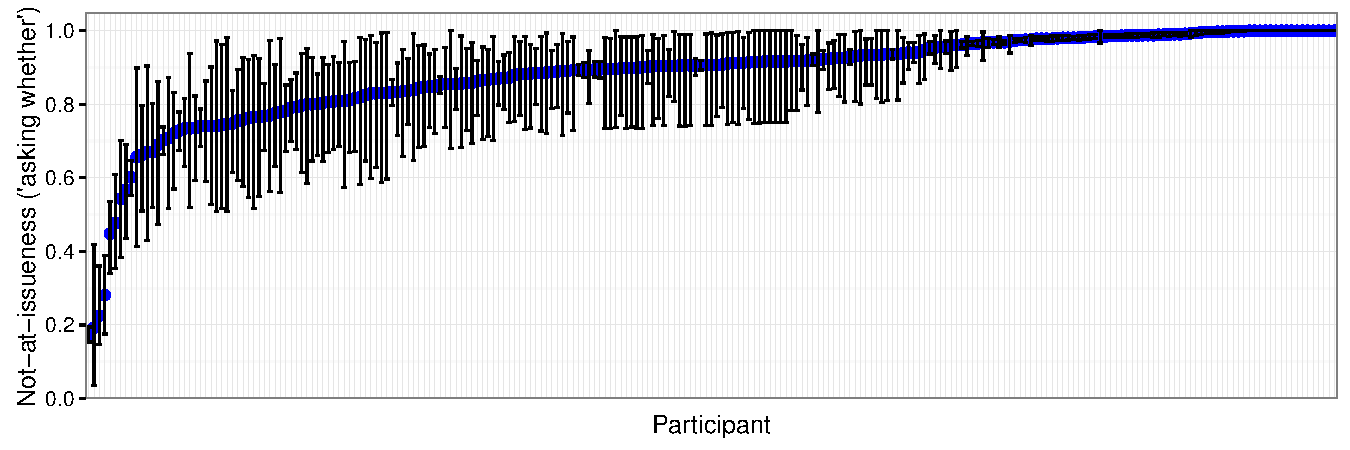
\includegraphics[width=16cm]{../results/exp1b/graphs/ai-subjectmeans}
%
%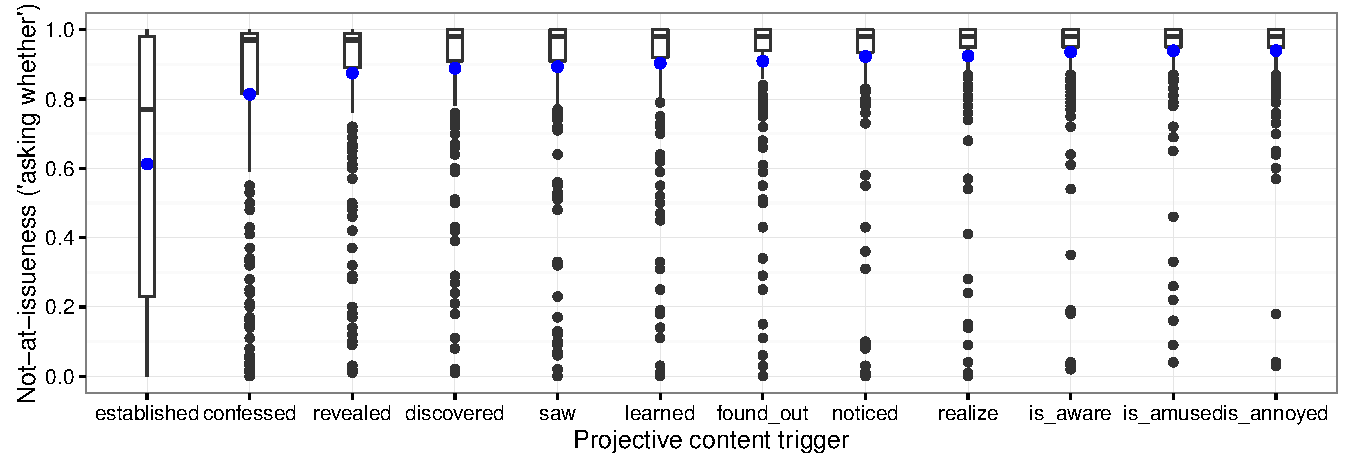
\includegraphics[width=16cm]{../results/exp1b/graphs/boxplot-not-at-issueness}
%
%\end{center}
%\caption{At-issueness by participant (top panel) and projective content trigger (bottom panel)}
%\label{f-ai-1b}
%\end{figure}


\subsubsection{Discussion}

Exp.~1b was designed to explore projection variability of the contents of the clausal complements of 12 (semi-)factive predicates and to further test the Projection Principle. Exp.~1b replicated the key findings of Exp.~1a: there is evidence for variability in the extent to which projective content projects and for a clear role for at-issueness in projectivity.

Like Exp.~1a, Exp.~1b revealed both by-expression and by-participant projection variability, but there was no evidence in Exp.~1b of by-lexical content variability. This difference between the experiments may be due to a number of factors. First, different lexical contents were included in the two experiments and it is possible that the lexical contents in Exp.~1a were more heterogeneous than those in Exp.~1b. Second, the lexical contents uniformly instantiated the contents of clausal complements in Exp.~1b, but a quite varied set of projective contents in Exp.~1a, which may contribute to the variability observed between the lexical contents. Third, recall that in Exp.~1b, each lexical content was paired with every target expression, whereas in Exp.~1a, each lexical content was paired with only a subset of target expressions. As a result, there were 3-21 data points per lexical content/expression combination in Exp.~1b, but 12-78 data points per lexical content/expression combination in Exp.~1a. This difference in number of ratings obtained may have contributed to the observed difference between the two experiments in by-lexical content variability. The role of the lexical contents in projectivity merits further investigation, which we leave to future research. 

The results of Exp.~1a and 1b also differed in the effects of block order on ratings: block order mattered in Exp.~1b, but not in Exp.~1a. The intricate ways in which task demands affect subsequent tasks also deserve further investigation, which we leave to future research.

A final comparison of the two experiments concerns the ratings obtained for the predicates {\em discover} and {\em be annoyed}, which were included in both experiments. Taking into account confidence intervals, the projectivity and at-issueness ratings for each predicate were indistinguishable in Exps.~1a and 1b: the projectivity means were .86 and .85 for {\em discover} for .96 and .92 for \emph{be annoyed}, respectively; the at-issueness means were .87 and .89 for \emph{discover} and .97 and .94 for \emph{be annoyed}, respectively. Furthermore, the small but significant difference in the projectivity of the contents of the clausal complements of the two predicates was maintained across the two experiments. This observation suggests that participants' responses were not substantially influenced by the other items they encountered, and that the `certain that' and `asking whether' diagnostics are stable methods for estimating projectivity and at-issueness, respectively.

\subsection{Summary and discussion of Experiments 1a and 1b}\label{s-summary1a1b}

Exps.~1a and 1b were designed to explore projection variability and the relation between projection and at-issueness for projective contents associated with 19 English expressions, as per the two research questions in (\ref{questions}). Regarding the first research question, the two experiments provided robust empirical evidence for variability across the 19 projective contents. In Exp.~1a, the projective contents associated with NRRCs, nominal appositives, {\em be annoyed}, possessive noun phrases and {\em know} were robustly projective and indistinguishable from one another in their projectivity. The projective contents associated with {\em stop, discover} and {\em be stupid to} were significantly less projective than the aforementioned projective contents (marginally so for the {\em stop/know} pair). And the prejacent of {\em only} was significantly less projective than all other projective contents. In Exp.~1b, the contents of the complements of {\em be annoyed, be amused, notice, be aware, realize, see, find out} and {\em learn} were robustly projective and indistinguishable from one another in their projectivity, and the content of the complement of {\em discover} was slightly less projective than the aforementioned 8 predicates. The contents of the complements of {\em reveal, confess} and {\em establish} were significantly less projective than that of the other 9 predicates, and of each other. 

An implicit assumption in the literature, reflected in distinctions such as those between `hard' and `soft' triggers, or between `factive' and `semi-factive' predicates, is that variable projectivity is categorical and, in particular, that there is a binary categorical distinction. Some of the observed distinctions in projection variability align with such commonly-assumed distinctions. For instance, the content of the complement of the cognitive `semi-factive' predicate {\em discover} and the pre-state implication of {\em stop}, both considered `soft' triggers, were significantly less projective than the content of the complement of the emotive `factive' predicates {\em be annoyed} and {\em be amused}, typically considered `hard' triggers (e.g., \citealt{abusch10}, though see \citealt{abrusan2011,abrusan2016}). Furthermore, the predicate {\em know} is often considered `factive' but has also been suggested to show some parallels with `semi-factives' and `soft' triggers (see, e.g., \citealt{kiparsky-kiparsky71,levinson83,simons01,chemla09b,beaver-geurts-sep}). Even though in Exp.~1a the content of the complement of {\em know} was more projective than the content of the complement of {\em discover}, and statistically indistinguishable in projectivity from the content of the complement of the `hard' triggering `factive' {\em be annoyed}, the mean projectivity of the content of the complement of {\em know} (.92) was numerically lower than that of {\em be annoyed} (.92).

Overall, however, the results of Exps.~1 do not provide empirical support for a binary categorical distinction in projectivity. For one, in both experiments, the projective content was divided by its relative projectivity into more than two classes. Second, even if the projective content in the two experiments could be divided up into just two classes, the observed distinctions in projection variability do not reflect commonly assumed divisions between `soft' and `hard' triggers, or between `factive' and `semi-factive' predicates. For instance, the projective content associated with {\em only} was significantly less projective than the contents of other expressions typically taken to be `weak' triggers. And the projectivity of the contents of the complements of the `hard' triggering emotive `factive' predicates {\em be annoyed} and {\em be amused} was indistinguishable in Exp.~1b from that of the contents of the complements of the `soft' triggering `semi-factive' predicates {\em notice, be aware, realize, see, find out} and {\em learn}. Furthermore, the contents of the complements of the `semi-factive' predicates {\em reveal, confess} and {\em establish} were significantly less projective than those of the previously mentioned `semi-factive' predicates, as well as each other.\footnote{While the content of the complement of {\em reveal} has generally been considered entailed and projective content (\citealt{hooper1974,melvold1991}), the previous literature is not always in agreement about the status of the contents of the complements of {\em confess} and {\em establish}. For {\em establish}, \citet{wyse} took the content of its complement to be projective, but \citet{swanson2012} classified the content as entailed, but not projective -- interestingly, he proposed the same for {\em discover}. The results of Exp.~1b suggest that the content of the complement of {\em establish} is projective content, compared to, for instance, non-projective main clauses -- and likewise for {\em discover}. For {\em confess}, authors generally take the content of its complement to be projective (e.g., \citealt{reis1973,melvold1991,schultz2003,swanson2012,karttunen2016}; cf.\ \citealt{wyse}), but \citet{swanson2012} suggested that the content of the complement is not entailed, giving a variant of the example in (i). (In Swanson's original example, {\em confess} had a {\em to-}infinitive as complement.)

\begin{exe}
\exi{(i)} She confessed that she took the money, but later recanted. It turned out that she had been trying to cover up a friend's mistake. \hfill (adapted from \citealt[1540]{swanson2012})
\end{exe}
%The idea that the content of the clausal complement of {\em confess} is not entailed is also supported by the acceptability of sentences with {\em falsely confessed} (as readily shown by a Google search), like (\ref{falsely}):
%
%\begin{exe}
%\ex\label{falsely} At that point, he said, he falsely confessed that he had taken \$10 from an undercover officer in a marijuana sale.\footnote{\url{http://www.nytimes.com/1985/04/22/nyregion/youth-s-charges-of-torture-by-an-officer-spur-inquiry.html}}
%\end{exe}
%However, the attitude holder in (\ref{confess}) recants the content of the complement of {\em confess}, i.e., she revises her beliefs about the content. As such, (\ref{confess}) does not seem the best kind of example for identifying whether the content of the complement of {\em confess} is entailed. Clearer examples that show that the content of the complement of {\em confess} is not entailed are not difficult to find. Consider, for instance, the naturally occurring example in (\ref{confess2}):
%
%\begin{exe}
%\ex\label{confess2} Bagley initially confessed that he took the goods, then later denied the thefts, blaming them on a “shady” acquaintance.\footnote{\url{http://nypost.com/2013/04/08/pretty-little-liars-actor-pleads-guilty-to-misdemeanor-petit-larceny/}}
%\end{exe}
Swanson's example is reminiscent of examples like (ii), which are discussed in the literature about whether the content of the complement of {\em know} is entailed:
\begin{exe}
\exi{(ii)} Everyone knew that stress caused ulcers, before two Australian doctors in the early 80s proved that ulcers are actually caused by bacterial infection. \hfill (\citealt[501]{hazlett2010})
\end{exe}
The question of whether `(semi-)factive' attitude predicates differ in the extent to which the content of their clausal complement is entailed is interesting, but outside the scope of this paper.} In sum, the observed projection variability does not provide empirical support for a categorical binary distinction along the lines of `soft' vs.\ `hard' triggers, or `factive' vs.\ `semi-factive' predicates.

We do find support for Beaver et al.'s 2017:281 prediction that projective content that does not have Obligatory Local Effect is more robustly not-at-issue and more robustly projective than content that has Obligatory Local Effect. In Exp.~1a, the projective content associated with NRRCs, nominal appositives and possessive noun phrases were among the four most projective and most not-at-issue of the 9 projective contents tested (see Figure \ref{fig:f-proj-ai-1a}). Whereas the content of the complement of the emotive `factive' {\em annoyed} was also robustly projective and not-at-issue, the other projective contents that have Obligatory Local Effect were less projective and not-at-issue. This finding is consistent with the hypothesis that projective content that does not have Obligatory Local Effect is not at-issue and, therefore, projects robustly.

Finally, recall that \citet{xue-onea11} found that the content of the complement of the German predicate {\em wissen} `know' was less projective than that of {\em erfahren} `find out'. In our experiments, by contrast, the mean projectivity ratings of the contents of the complements of {\em discover} and {\em find out} were lower  than that of the content of the complement of {\em know} ({\em discover}: .86 Exp.~1a, .85 Exp.~1b; {\em find out}: .88 Exp.~1b; {\em know}: .92 Exp.~1a). While these findings may be suggestive of cross-linguistic variation, it is important to note that there are several differences between \citetpos{xue-onea11} experiment and ours: in their study, the predicates were embedded in the antecedents of conditionals rather than in polar questions; participants were asked to judge whether it is possible that the content of the complement is false rather than whether the speaker is certain of the content of the complement; and, finally, the projective contents were instantiated with different lexical contents. Exploring potential cross-linguistic variation in projectivity is an important area for future research.

Regarding the second research question, whether at-issueness plays a role in projectivity, Exps.~1a and 1b both provided empirical support for such a role, as predicted by  \citepos{brst-ar} Projection Principle. Specifically, we found that the information-structural status of the 19 projective contents tested was related to the projectivity of these contents. This finding significantly substantiates the ``clear correlation between projection and not-at-issueness'' that was suggested in \citealt[180]{xue-onea11} based on two pilot experiments involving four German expressions associated with projective content. Furthermore, the findings of Exps.~1a and 1b both suggest that the projectivity of projective content is also influenced by the expression that the projective content is associated with, by the lexical content that the projective content is instantiated with and by the speaker of American English that judges the projectivity.  Thus, in sum, the findings of Exps.~1a and 1b suggest that the projectivity of utterance content is a function of several factors. We discuss the implications of these findings for analyses of projection in section \ref{s5}, after further testing the Projection Principle in Exps.~2.

Our exploration of the Projection Principle in Exps.~1 relied on exploring the at-issueness of projective content using the `asking whether' diagnostic. This diagnostic was chosen to assess at-issueness because i) it was used in previous research on at-issueness (e.g., \citealt{amaral-etal07,tonhauser-sula6}) and ii) the diagnostic is suitable to diagnose the at-issueness of projective content associated with expressions realized in polar questions (recall that the expressions were embedded in polar questions to assess projectivity). However, a potential worry is that the `asking whether' at-issueness diagnostic and the `certain that' projectivity diagnostic seem to mirror each other. After all, if Patrick, after uttering the polar question in (\ref{stim}), is taken to be certain that Martha's new car is a BMW, then he is presumably not asking whether her new car is a new BMW, and if he is taken to be asking whether Martha's new car is a BMW, then he is presumably not certain that her new car is a BMW.

\begin{exe}

\exi{(\ref{stim})} Patrick asks: {\em Was Martha's new car, a BMW, expensive?} 

\begin{xlist}
\ex `certain that' question: Is Patrick certain that Martha's new car is a BMW?

\ex `asking whether' question: Is Patrick asking whether Martha's new car is a BMW?

\end{xlist}

\end{exe}
Luckily, several different diagnostics have been used in the literature to diagnose at-issueness (see, e.g., \citealt{tonhauser-sula6}; for further discussion see section \ref{s-disc2}). The second pair of experiments, Exps.~2a and 2b, explored the at-issueness of the 19 projective contents using a different diagnostic for at-issueness to establish that the empirical support for the Projection Principle obtained in Exps.~1 is not merely an artifact of the at-issueness diagnostic used.

\section{Confirming the role of at-issueness in projectivity}\label{s4}

In Exp.~2, the at-issueness of the 19 projective contents was explored with a diagnostic that relies on the assumption that at-issue and not-at-issue content differ in the extent to which it is up for debate and can be directly assented/dissented with. For previous uses of diagnostics that rely on this assumption see, e.g., \citealt{amaral-etal07,xue-onea11,murray2014,anderbois-etal2015,destruel-etal2015,tonhauser-sula6} and \citealt{syrett-koev2015}. The 3-turn dialogue in (\ref{sure}) illustrates how the diagnostic was set up, using the appositive content associated with nominal appositives as an example. The speaker of the first turn, here Fred, utters an indicative sentence with the target expression, here a nominal appositive, and thereby commits himself to various utterance contents, including the appositive content that Martha's new car is a BMW. The speaker of the second turn, here Carla, utters the question {\em Are you sure?}, thereby challenging some content of the first speaker's utterance. In the third turn, the speaker of the first turn utters an indicative sentence in which the content to be diagnosed for at-issueness, here the appositive content of the first turn, realizes the content of the clausal complement of {\em sure}, thereby identifying it as the content that they took the second speaker to be challenging. 

\begin{exe}
\ex\label{sure} 
\begin{xlist}
\exi{Fred:} Martha's new car, a BMW, was expensive.

\exi{Carla:} Are you sure?

\exi{Fred:} Yes, I am sure that Martha's new car is a BMW.
\end{xlist}
\end{exe}
To assess whether participants take the 19 projective contents to be at-issue, i.e., up for debate and a possible target of the second speaker's dissent, we asked them to respond to the question of whether the first speaker answered the question of the second speaker, using a slider from `no' to `yes'. In (\ref{sure}), for instance, the question participants responded to was: {\em Did Fred answer Carla's question?}. A `no' response was taken to indicate that the participant took Carla to have challenged a different content and Fred to therefore not have answered Carla's question; in this case, the projective content was not at-issue. A `yes' response, on the other hand, was taken to indicate that the participant took Carla to have challenged the projective content and Fred to have answered Carla's question, and, therefore, that the projective content was at-issue.\footnote{As mentioned above, our second at-issueness diagnostic relies on the assumption that at-issue and not-at-issue content differ in the extent to which it is up for debate and can be directly assented/dissented with. Our diagnostic differs from diagnostics used in prior research based on the same assumption because we wanted to explore the at-issueness of a broader set of projective contents and, in particular, ones that are not independent of the main clause content.  \citet{xue-onea11}, for instance, presented participants with indicative sentences with the target expressions, as did we, but asked participants to choose between (German versions of) `Yes, and \ldots' followed by a clause that denies the relevant content and `No, (but) \ldots' followed by a clause that denies the relevant content.  \citet{syrett-koev2015} also presented participants with indicative sentences with the target expressions, but asked participants to choose between a direct dissent utterance `No, \ldots' followed by a clause that denies the relevant content and a direct dissent utterance `No, \ldots' followed by a clause that denies the main clause content. These diagnostics are unsuitable for expressions that entail the projective content they are associated with: for instance, these diagnostics are not suitable for an indicative sentences with {\em know}, like {\em Billy knows that Martha has a new BMW}, because it is not possible to agree with the truth of the main clause content and simultaneously deny the truth of the content of the complement clause (one of the response options in \citepos{xue-onea11} diagnostic) and because denying the truth of the content of the complement also denies the truth of the main clause content (one of the response options in \citepos{syrett-koev2015} diagnostic).}

The at-issueness diagnostic used in Exp.~2 thus differs from the one used in Exp.~1 in several ways: i) the target expressions are realized in indicative sentences rather than in polar questions, i.e., not embedded under an entailment-canceling operator; ii) the diagnostic relies on the assumption that at-issue and not-at-issue content differ in the extent to which it is up for debate and can be dissented with, rather than in the extent to which it and its negation partition the context set; and iii) participants were asked to rate whether an interlocutor's utterance answered another interlocutor's question, rather than whether a speaker is asking about a particular content. Because the target expressions in Exp.~2 are not realized in the scope of an entailment-canceling operator, we cannot collect projectivity ratings for the projective contents associated with the target expressions. To assess whether the at-issueness of the 19 projective contents under this second diagnostic plays a role in their projectivity, we collected at-issueness ratings for the same combinations of target expressions and lexical contents as in Exp.~1, and then related the mean at-issueness rating of each combination to the mean projectivity rating of the same combination from Exp.~1. If projectivity is a function of at-issueness, we expect this second, substantially different, diagnostic to confirm the relation between projectivity and at-issueness observed in Exp.~1. We present the results of Exps.~2a and 2b in sections \ref{s-exp2a} and \ref{s-exp2b}, and then discuss the results and compare the two at-issueness diagnostics in section \ref{s-disc2}.

\subsection{Experiment 2a}\label{s-exp2a}

Exp.~2a explored the at-issueness of the 9 projective contents that we explored in Exp.~1a, i.e., the contents of NRRCs and nominal appositives, the possession implication of possessive noun phrases, the prejacents of {\em only} and {\em be stupid to}, the pre-state implication of {\em stop} and the contents of the clausal complements of {\em be annoyed, discover} and {\em know}, using the {\em Are you sure?}~diagnostic introduced above.

\subsubsection{Methods}\label{s-methods-2a}

\paragraph{Participants.} 250 participants with U.S.\ IP addresses and at least 97\% of previous HITs approved were recruited on Amazon's Mechanical Turk platform (ages: 20-77; median: 30). They were paid 30 cents for their participation.


\paragraph{Materials.} Stimuli consisted of written 3-turn dialogues between two individuals, as in (\ref{sure}). In the target stimuli, the first turn of each dialogue consisted of an indicative sentence that realized one of the 9 target expressions. The projective contents of these 9 target expressions were instantiated by the same 17 lexical contents as in Exp.~1a (see section \ref{s-methods-1a}). Thus, there were a total of 43 indicative sentences with target expressions that realized the first turn of the target stimuli. The second turn of the target stimuli consisted of a second speaker's {\em Are you sure?}~question and the third turn consisted of an utterance by the first speaker in which {\em Yes, I am sure that} was followed by a clause that realized the projective content to be diagnosed.

As in Exp.~1a, there were 17 control stimuli in Exp.~2a: in the control stimuli, the first turn consisted of an indicative sentence that realized one of the 17 lexical contents and, in the third turn, the clause that realized the lexical content was the complement of {\em sure}. A sample control dialogue is shown in (\ref{sure2}). The full set of stimuli of Exp.~2a is provided in Appendix \ref{a-exp1a-2a-stimuli}.


\begin{exe}
\ex\label{sure2}
\begin{xlist}
\exi{Sandra:} Martha has a new BMW.

\exi{Carl:} Are you sure?

\exi{Sandra:} Yes, I am sure that Martha has a new BMW.
\end{xlist}
\end{exe}

For each participant, a set of 15 stimuli was randomly created: each set contained a target stimulus for each of the 9 target expressions (the projective content associated with each expression was instantiated by a unique lexical content) and 6 control stimuli (with unique lexical contents as well, for a total of 15 unique lexical contents). Trial order was randomized for each participant.


\paragraph{Procedure.} Participants were told to imagine that they are at a party and, upon walking into the kitchen, overhear a short conversation between two people. Participants were then presented with the 15 stimuli in random order and were asked to assess, for each stimulus, whether the speaker of the first/third turn answered the question of the speaker of the second turn. Participants gave their responses on a slider marked `no' at one end and `yes' at the other, as shown in Figure \ref{f-trial-exp2a}. A `yes' response was taken to indicate that the relevant content was at-issue and a `no' response that the relevant content was not at-issue. To explore the hypothesis that projectivity and not-at-issueness are positively related, `yes' responses were coded as `0' and `no' responses as `1'. 

\begin{figure}[!h]
\begin{center}
\fbox{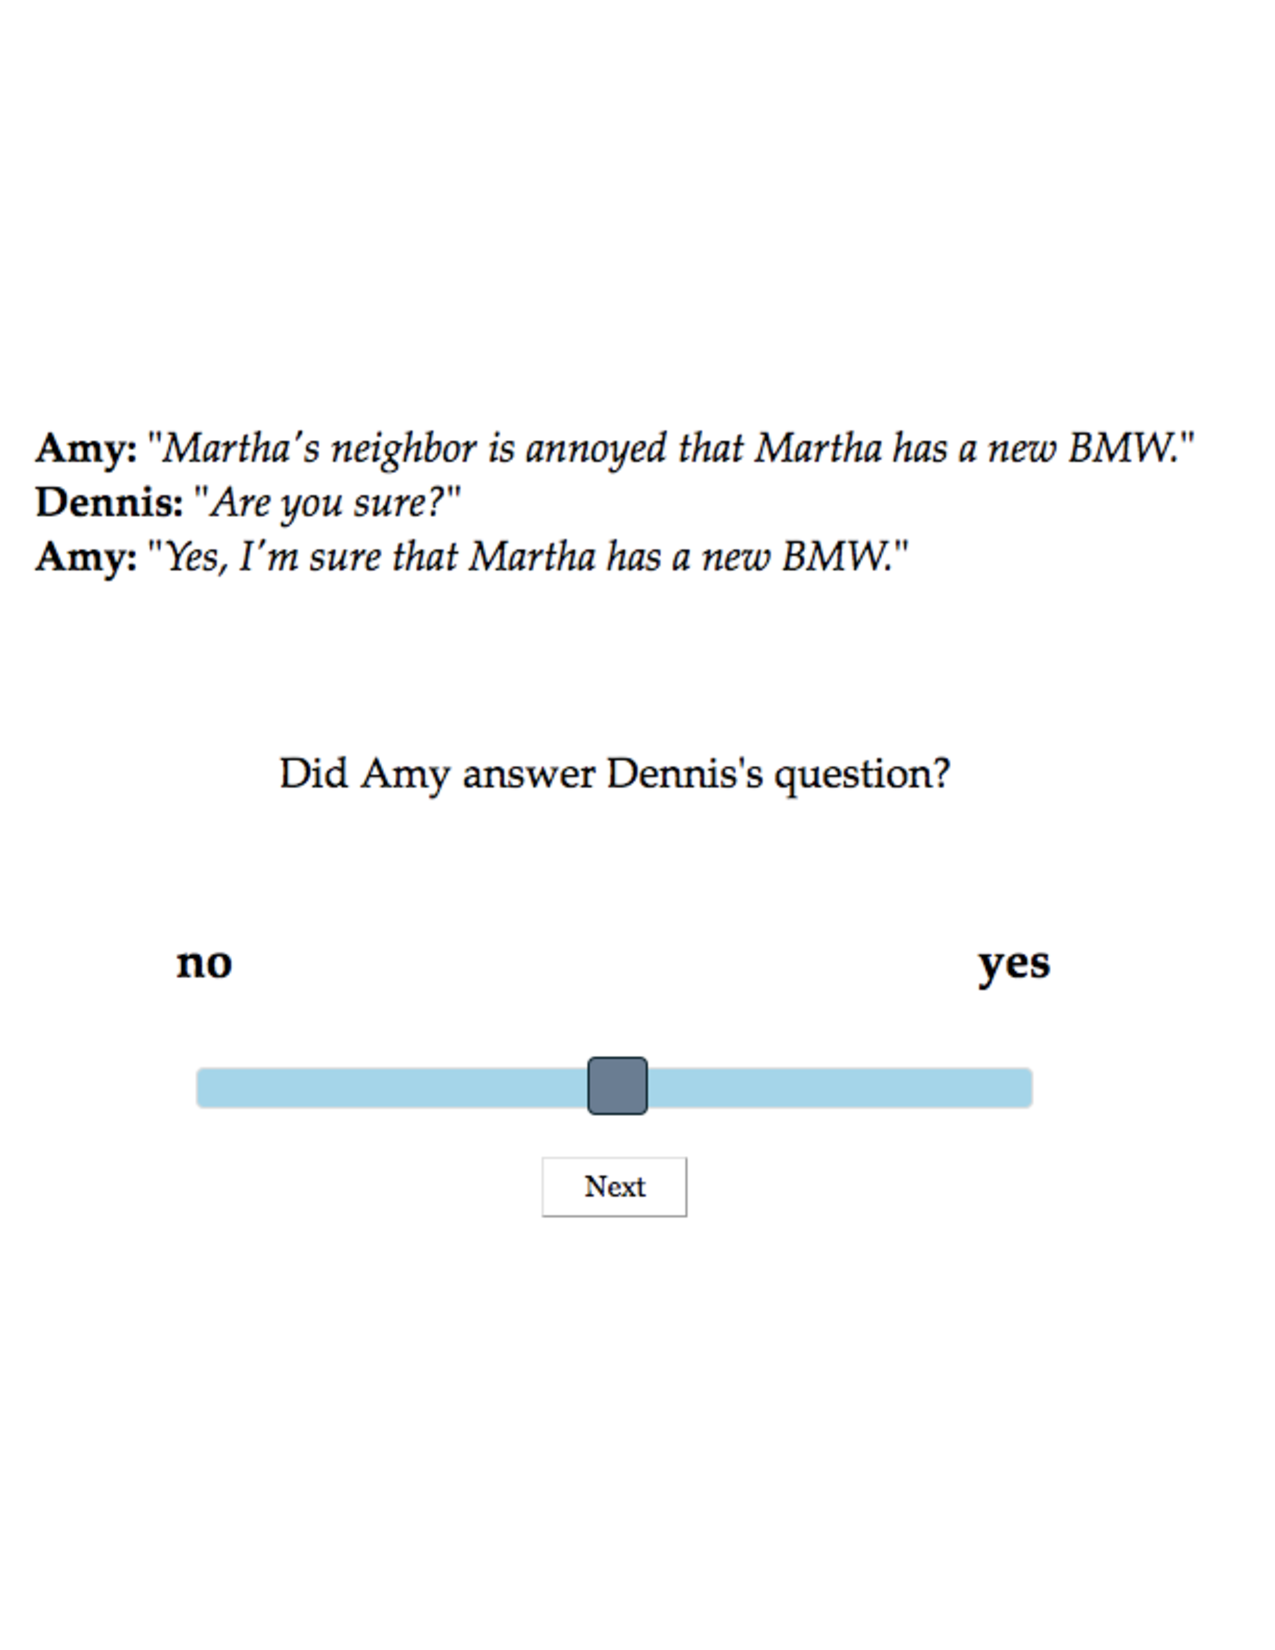
\includegraphics[width=12cm]{figures/exp2-trial}}
\end{center}
\caption{A sample trial in Exp.~2}
\label{f-trial-exp2a}
\end{figure}

After completing the experiment, participants filled out the same optional survey as in Exps.~1 about their age, their native language(s) and, if English is their native language, whether they are a speaker of American English (as opposed to, e.g., Australian or Indian English). To encourage them to respond truthfully, participants were told that they would be paid no matter what answers they gave in the survey.

\paragraph{Data exclusion.} Prior to analysis, we excluded the data from 6 participants who did not self-identify as native speakers of American English. Inspection of the response means of the remaining 244 American-English speaking participants to the 6 control stimuli revealed 6 participants whose response means were more than 3 standard deviations above the group mean (which was .04). Further inspection revealed that these participants' responses were systematically higher than the group mean and involved 14 of the 17 lexical contents, suggesting that these participants did not attend to the task or interpreted the task differently. The data from these 6 participants were also excluded, leaving data from 238 participants (ages 20-77; median: 30).


\subsubsection{Results}

Mean projectivity ratings obtained for target expression/lexical content combinations in Exp.~1a are shown in \figref{fig:f-proj-ai-2a} as a function of their mean not-at-issueness ratings obtained in Exp.~2a ($r =$ .84; when not collapsing across lexical contents $r =$ .6). There is a clear relationship between at-issueness and projectivity: the more not-at-issue a projective content is, as measured by the second at-issueness diagnostic, the more projective it is.

\begin{figure}[!h]

\begin{center}
%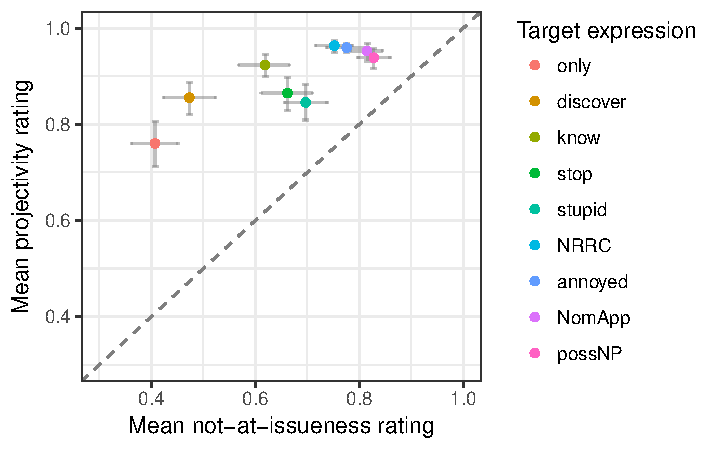
\includegraphics[width=12cm]{../results/exp2a/graphs/ai-proj-bytrigger}
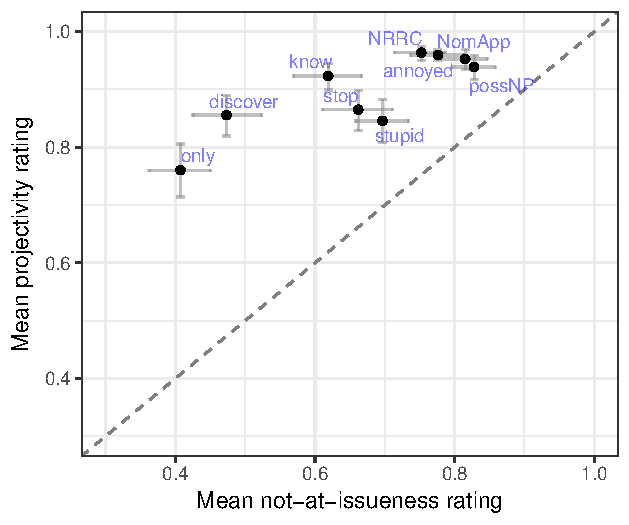
\includegraphics[width=10cm]{../results/exp2a/graphs/ai-proj-bytrigger-labels}
\end{center}

\caption{Mean projectivity against mean not-at-issueness by target expression. Error bars indicate bootstrapped 95\% confidence intervals. Dashed line indicates identical values on at-issueness and projectivity scales.}
\label{fig:f-proj-ai-2a}
\end{figure}


The observed relationship was borne out statistically. We conducted a similar mixed-effects linear regression analysis as we did for Exp.~1a, predicting projectivity from a centered fixed effect of at-issueness and random by-lexical content intercepts. This model differed from that in Exp.~1a in the following three ways: i) because we predicted projectivity ratings given by one group of participants (Exp.~1a) from at-issueness ratings given by another group of participants (Exp.~2a), by-participant random effects were not included. Instead, the model predicted projectivity \emph{means}  from  at-issueness \emph{means} (collapsing across participants but not lexical contents or target expressions, yielding 43 data points); ii) there was no fixed effect of block because block was not manipulated; iii) by-expression random effects and random by-lexical content slopes for at-issueness were not included because likelihood ratio tests revealed that the only random effect justified by the data was that of by-lexical content intercepts ($SD$ = .04, $p < $ .05). The model we report here thus only contained one fixed effect (at-issueness) and one random effect (by-lexical content intercepts).

We observed a significant main effect of at-issueness, such that more not-at-issue expression/lexical content combinations received higher projectivity ratings ($\beta$ = 0.29, $SE$ = 0.06, $t$ = 5.21, $\chi^2(1)$ = 20.94, $p <$ .0001), replicating the at-issueness effect observed in the previous experiments.\footnote{In the model with the full random effects structure (random by-lexical content and by-expression intercepts and slopes for at-issueness), the effect of at-issueness was only marginally significant ($\beta$ = 0.25, $SE$ = 0.08, $t$ = 3.15, $\chi^2(1)$ = 3.51, $p <$ .07).  A post hoc power analysis using the simr package \citep{simr} revealed that this model had only 60.4\% power to detect an effect size of $\beta$ = .25, while the model with the simplified random effects structure had 99.8\% power to detect an effect size of $\beta$ = .29. This means that the dataset is not large enough to jointly estimate the effects of at-issueness and the random effects. However, the fact that at-issueness is a marginally significant predictor of projectivity even in this low-powered dataset provides further evidence for the relation between at-issueness and projectivity.}

\subsection{Experiment 2b}\label{s-exp2b}

Exp.~2b explored the at-issueness of the 12 projective contents that we explored in Exp.~1b, namely the contents of the clausal complements of the predicates {\em be amused, be annoyed, be aware, see, discover, notice, find out, realize, learn, establish, confess} and {\em reveal}, using the {\em Are you sure?}~diagnostic.

\subsubsection{Methods}

\paragraph{Participants.} 250 participants with U.S.\ IP addresses and at least 97\% of previous HITs approved were recruited on Amazon's Mechanical Turk platform (ages: 18-77; median: 29). They were paid 30 cents for their participation.

\paragraph{Materials.} As in Exp.~2a, the stimuli consisted of 3-turn dialogues between two individuals. In the target stimuli, the first turn of each dialogue consisted of an indicative sentence that realized one of the 12 predicates, as shown in (\ref{sure3}). The contents of the complements of these predicates were instantiated by the same 20 lexical contents as in Exp.~1b (see section \ref{s-methods-2a}), for a total of 240 target stimuli. The third turn of the target stimuli consisted of the first speaker's utterance of {\em Yes, I am sure that}, with the relevant projective content realized as the content of the complement of {\em sure}. 

\begin{exe}
\ex\label{sure3}
\begin{xlist}
\exi{Sandra:} Shirley is aware that Raul was drinking chamomile tea.

\exi{Carl:} Are you sure?

\exi{Sandra:} Yes, I am sure that Raul was drinking chamomile tea.
\end{xlist}
\end{exe}

As in Exp.~1b, there were 20 control stimuli in Exp.~2a: in the control stimuli, the first turn consisted of an indicative sentence that realized one of the 20 lexical contents and, in the third turn, the clause that realized the lexical content was the complement of {\em sure}. A sample control stimulus is shown in (\ref{sure4}).

\begin{exe}
\ex\label{sure4}
\begin{xlist}
\exi{Sandra:} Raul was drinking chamomile tea.

\exi{Carl:} Are you sure?

\exi{Sandra:} Yes, I am sure that Raul was drinking chamomile tea.
\end{xlist}
\end{exe}

For each participant, a set of 20 stimuli was randomly created: each set contained a target stimulus for each of the 12 target expressions (the projective content associated with each expression was instantiated by a unique lexical content) and 8 control stimuli (with unique lexical contents as well, for a total of 20 unique lexical contents). Trial order was randomized for each participant.

\paragraph{Procedure.} The procedure was the same as in Exp.~2a, described in section \ref{s-methods-2a}, except that participants completed 20 trials instead of 15.

\paragraph{Data exclusion.} Prior to analysis, we excluded the data from 6 participants who did not self-identify as native speakers of American English. Inspection of the response means of the remaining 244 American-English speaking participants to the 8 control stimuli revealed 6 participants whose response means were more than 3 standard deviations above the group mean (which was .05). Further inspection revealed that these participants' responses were systematically higher than the group mean and involved 18 of the 20 lexical contents, suggesting that these participants did not attend to the task or interpreted the task differently. The data from these 6 participants were also excluded, leaving data from 238 participants (ages 18-77; median: 30).


\subsubsection{Results}

Mean projectivity ratings obtained for target expression/lexical content combinations in Exp.~1b are shown in \figref{fig:f-proj-ai-2b} as a function of their mean not-at-issueness ratings obtained in Exp.~2b ($r =$ .54; when not collapsing across lexical contents $r =$ .28). While there appears to be an overall increase in projectivity with increasing not-at-issueness, as predicted by the Projection Principle, the relationship is clearly not linear, unlike in the previous experiments.

\begin{figure}[!h]

\begin{center}
%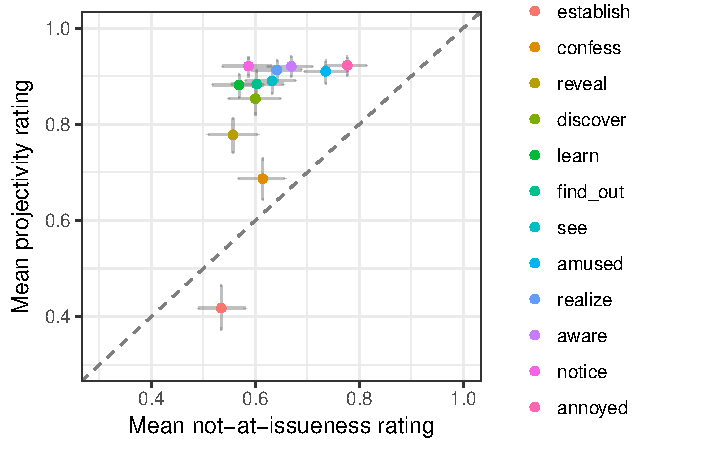
\includegraphics[width=12cm]{../results/exp2b/graphs/ai-proj-bytrigger}
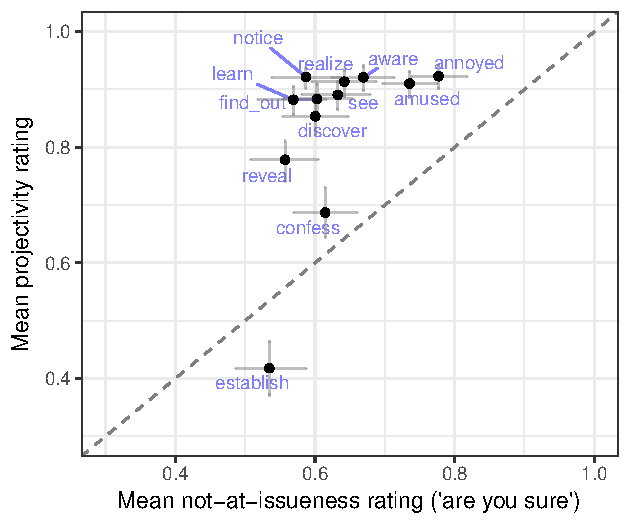
\includegraphics[width=10cm]{../results/exp2b/graphs/ai-proj-bytrigger-labels}
\end{center}

\caption{Mean projectivity against mean not-at-issueness by target expression. Error bars indicate bootstrapped 95\% confidence intervals. Dashed line indicates identical values on at-issueness and projectivity scales.}
\label{fig:f-proj-ai-2b}
\end{figure}


%Formula: mean_proj ~ cmean_ai + (1 | short_trigger)
%   Data: means_nomc
%
%     AIC      BIC   logLik deviance df.resid 
%  -554.1   -540.1    281.0   -562.1      236 
%
%Scaled residuals: 
%    Min      1Q  Median      3Q     Max 
%-3.0835 -0.5640  0.1461  0.6739  2.4186 
%
%Random effects:
% Groups        Name        Variance Std.Dev.
% short_trigger (Intercept) 0.020061 0.14164 
% Residual                  0.004494 0.06704 
%Number of obs: 240, groups:  short_trigger, 12
%
%Fixed effects:
%            Estimate Std. Error t value
%(Intercept)  0.83092    0.04112  20.209
%cmean_ai     0.03320    0.04014   0.827
%
%Correlation of Fixed Effects:
%         (Intr)
%cmean_ai 0.000 

A mixed effects linear regression predicting 240 mean projectivity ratings from mean at-issueness and random by-expression intercepts (the only random effect term justified in likelihood ratio tests, $SD$ = .07, $p <$ .0001) yielded no significant effect of at-issueness ($\beta$ = 0.03, $SE$ = 0.04, $t$ = 0.83, $\chi^2(1)$ = 0.68, $p >$ .4), but the sign of the coefficient went in the predicted direction.\footnote{A power analysis revealed that this model had 99\% power to detect an effect size for at-issueness of $\beta$ = .29 (i.e., an effect size comparable to that from Exp.~2a).  However, from \figref{fig:f-proj-ai-2b} it is already clear that the relation between at-issueness and projectivity in this experiment is not linear. A more principled analysis of the functional relationship between at-issueness and projectivity measures merits exploration, but is beyond the scope of this paper.   %We therefore conducted an analysis that included a restricted cubic spline with 1 knot instead of the simple linear predictor for at-issueness. Model comparison revealed that the spline was not justified. Thus, this can be taken as evidence that there is a lack of effect of at-issueness in Exp.~2b.}
}



\subsection{Summary and discussion of Experiments 2a and 2b}\label{s-disc2}

Exps.~2a and 2b were designed to further test the Projection Principle (research question \ref{questions}b) by exploring the at-issueness of the 19 projective contents using a second diagnostic for at-issueness. We found that at-issueness was a significant predictor of the projectivity of the 9 projective contents in Exp.~2a but not of the projectivity of the 12 projective contents in Exp.~2b. Thus, as summarized in the second column of Table \ref{t-summary}, we have obtained empirical support for the Projection Principle (see \citealt{brst-salt10,brst-ar}) for a broad range of projective contents using two distinct diagnostics for at-issueness. The two experiments also differed in which other factors were found to play a role in projectivity: as summarized in the remaining columns of Table \ref{t-summary} we observed random lexical content variability in Exp.~2a but not in Exp.~2b, and random target expression variability in Exp.~2b but not in Exp.~2a. These two findings further confirm what Exps.~1 already suggested, namely that the projectivity of a projective content is not merely a function of its at-issueness, but also of the lexical content that instantiates the projective content and the expression that the projective content is associated with. 

\begin{table}[h!]

\begin{center}
\begin{tabular}{p{1.8cm} | c | c c c | c c c c}
\toprule
& & \multicolumn{3}{c|}{Intercepts} & \multicolumn{3}{c}{Slopes for at-issueness}\\
Exp. (\# of data points) & At-issueness & Expression & Content & Participant & Expression & Content & Participant\\
\midrule
1a (1,890) & ** & *** & ** & *** & *** & *** & ***  \\ 

1b (2,820) & *** & *** & \emph{n.s.} &  *** & \emph{n.s.} & \emph{n.s.} & *** \\ 

2a (43) & *** & \emph{n.s.} & * & -- & \emph{n.s.} & \emph{n.s.} & -- \\ 

2b (240) & \emph{n.s.} & *** & \emph{n.s.} & --& \emph{n.s.} & \emph{n.s.} & -- \\ 
\bottomrule
\end{tabular}
\end{center}
\caption{Summary of findings in Exps.~1 and 2. `Expression' abbreviates target expression, `Content' abbreviates lexical content. `***' indicates significance at .0001, `**' at .01, `*' at .05, \emph{n.s} indicates no significance and `--' indicates `not applicable'.}\label{t-summary}
\end{table}

The implications of these findings for analyses of projection are discussed in section \ref{s5}. In the remainder of this section, we compare the two at-issueness diagnostics. 

\paragraph{Comparison of the at-issueness diagnostics used in Exps.~1 and 2.} The two diagnostics for at-issueness yielded different results in Exp.~1b and 2b about the relationship between at-issueness and projectivity. A comparison of the at-issueness of the 9 projective contents in Exps.~1a and 2a based on \figref{f-ai-a} reveals further differences. First, the contents generally received higher ratings on the `asking whether' diagnostic than on the {\em Are you sure?}~diagnostic (despite the main clause controls receiving roughly comparable ratings, with a mean rating of .02 on the `asking whether' and a mean rating of .03 on the {\em Are you sure?}~diagnostic). Second, there is greater variability in the not-at-issueness ratings on the {\em Are you sure?}~diagnostic  than on the `asking whether' diagnostic. Third, the spread of the mean ratings is greater on the {\em Are you sure?}~diagnostic than on the `asking whether' diagnostic. And, finally, the relative not-at-issueness of some of the contents differs: the prejacent of {\em stop}, for instance, is the least not-at-issue content on the `asking whether' diagnostic but not on the {\em Are you sure?}~diagnostic. Similar differences emerge from a comparison of the results of the two at-issueness diagnostics in Exp.~1b and 2b, shown in Appendix \ref{a-ai1b2b}. 

\begin{figure}[h!]
\begin{center}

\subfloat[][Boxplot of not-at-issueness ratings in Exp.~1a.]{ 
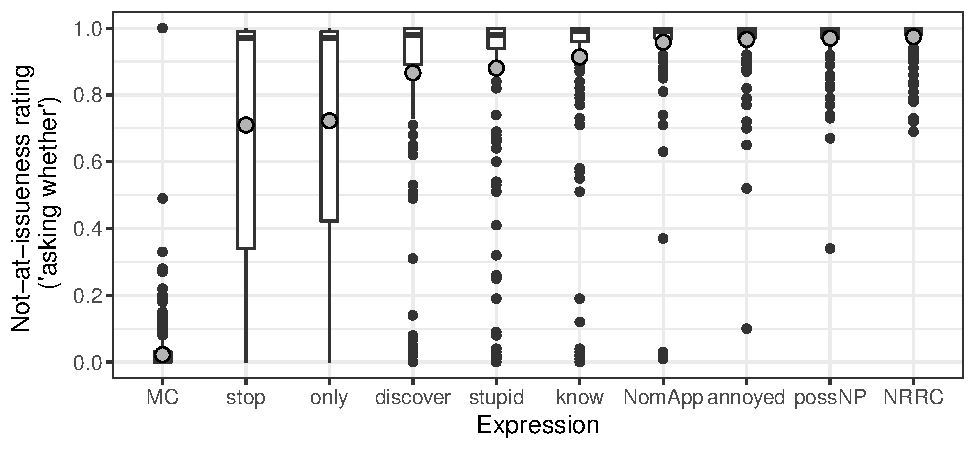
\includegraphics[width=12cm]{../results/exp1a/graphs/boxplot-not-at-issueness-with-MCs}
\label{fig:aimeans-1a}
}

\subfloat[][Boxplot of not-at-issueness ratings in Exp.~2a.]{ 
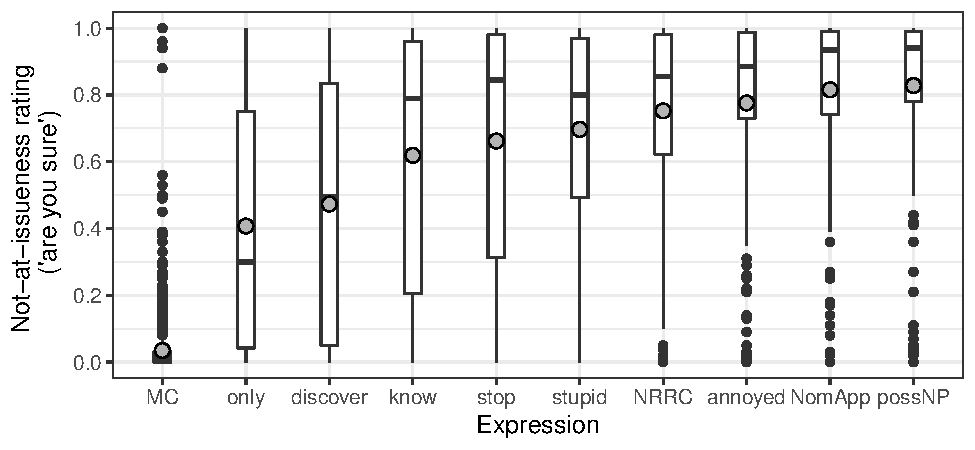
\includegraphics[width=12cm]{../results/exp2a/graphs/boxplot-not-at-issueness-with-MCs}
\label{fig:aimeans-2a}
}

\end{center}
\caption{Not-at-issueness ratings by expression, including main clauses and collapsing across lexical contents, in Exp.~1a (top panel) and Exp.~2a (bottom panel). Grey dots indicate means and notches indicate medians.}
\label{f-ai-a}
\end{figure}

%Some of the same differences emerge from a comparison of the results of the two at-issueness diagnostics in Exp.~1b and 2b. As shown in \figref{f-ai-b}, the 12 projective contents generally received higher not-at-issueness ratings on the `asking whether' diagnostic than on the {\em Are you sure?}~diagnostic, and there is greater variability in the not-at-issueness ratings on the {\em Are you sure?}~diagnostic  than on the `asking whether' diagnostic. There are also again differences in the relative not-at-issueness of projective contents across the two diagnostics: for instance, whereas the content of the complement of {\em notice} is more not-at-issue than that of {\em confess} on the `asking whether' diagnostic, the same is not true on the {\em Are you sure?}~diagnostic.

The fact that both diagnostics for at-issueness, despite these differences, provide evidence for the relationship between at-issueness and projectivity  further strengthens the empirical support for the Projection Principle. Furthermore, there is also evidence that the two ways of operationalizing at-issueness measure the same underlying concept. Consider \figref{fig:ai-correlation}, which shows mean at-issueness ratings for target expressions obtained in Exp.~1 as a function of their mean at-issueness ratings obtained in Exp.~2. There is a clear relationship between the two diagnostics: the more not-at-issue projective content is on the {\em Are you sure?}~diagnostic, the more not-at-issue it is on the `asking whether' diagnostic. The correlation at the target expression level (collapsing across contents) was $r$ = .62. Not collapsing across contents, i.e., taking into account variability between lexical contents, the correlation was still $r$ = .31. The correlation was greater for the heterogeneous target expressions (Exps.~a, $r$ = .70) than for the homogeneous target expressions (Exps.~b, $r$ = .56).\footnote{The observed relationship was also borne out statistically in a mixed effects linear regression predicting mean at-issueness in Exps.~2 (collapsing across participants but not across target expressions or lexical contents) from centered fixed effects of mean at-issueness in Exps.~1, centered sub-experiment (a vs.~b), their interaction, and random by-lexical content random intercepts. There was a significant main effect of at-issueness ($\beta$ = 0.38, $SE$ = 0.07, $t$ = 5.58, $p <$ .0001), suggesting that the at-issueness measures are indeed good predictors of one another. The main effect of sub-experiment did not reach significance  ($\beta$ = -0.03, $SE$ = 0.02, $t$ = -1.51, $p <$ .13). However, there was a significant interaction between Exp.~1 at-issueness and sub-experiment ($\beta$ = -0.47, $SE$ = 0.21, $t$ = -2.27, $p <$ .05). Simple effects analysis revealed that this interaction was due to a difference in slope between sub-experiments: Exp.~1a at-issueness was a better predictor of Exp.~2a at-issueness ($\beta = 0.77$) than Exp.~1b at-issueness was of Exp.~2b at-issueness ($\beta = 0.31$), capturing the correlations reported above. There was no random by-lexical content variation  ($SD$ = 0.00).} In short, these findings are compatible with the two diagnostics both measuring at-issueness, though the imperfect correlation suggests that other factors are also contributing to participants' ratings.

\begin{figure}[!h]
\begin{center}

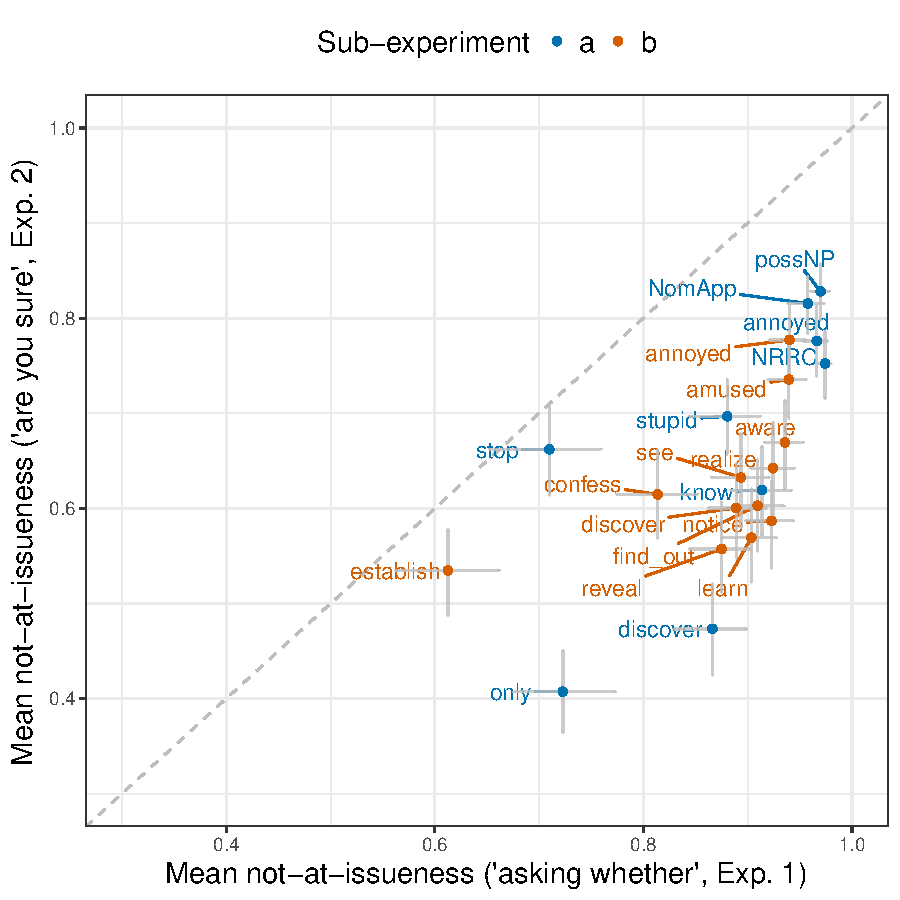
\includegraphics[width=12cm]{../results/ai-meta-analysis/graphs/correlation-bytrigger}

\end{center}
\caption{Mean not-at-issueness ratings for each target expression in Exps.~1 and 2. Colors indicate the subexperiment that the target expression occurred in (blue for subexperiments a and red for subexperiments b). Error bars indicate bootstrapped 95\% confidence intervals. Dashed line indicates identical values on at-issueness scales.}
\label{fig:ai-correlation}
\end{figure}


To assess the observed differences, the extent to which the two diagnostics measure the theoretical concept of at-issueness, i.e., the extent to which the experimental tasks constitute reasonable operationalizations of at-issueness, needs to be evaluated. And this is where the trouble starts: in an ideal world, diagnostics for at-issueness or, rather, the assumptions about at-issue versus not-at-issue content that diagnostics rely on, would have been derived from a theoretical characterization of the concept of at-issueness. But research on at-issueness did not proceed in this orderly fashion;  formal characterizations of at-issueness that go beyond calling at-issue content the `main point' and not-at-issue content `backgrounded' or `secondary' have only recently been developed. On one prominent characterization, at-issue content is proposed to be added to the common ground, whereas not-at-issue content is imposed on the common ground (e.g., \citealt{murray2014,anderbois-etal2015}); on another, at-issue utterance content is (minimally) relevant to the Question Under Discussion of the utterance (e.g., \citealt{brst-salt10,brst-ar}). 

We are not aware of experimental research that uses an at-issueness diagnostic that relies on the assumption of our `asking whether' diagnostic, that at-issue and not-at-issue content differ in the extent to which it and its negation partition the context set. Our {\em Are you sure?}~diagnostic, by contrast, relies on the assumption that at-issue and not-at-issue content differ in the extent to which it is up for debate and can be dissented with. Where comparison is possible, our findings on this diagnostic are similar to those of other research that used diagnostics that relied on this assumption. As reported in section \ref{s1}, \citet{amaral-etal11} found that the prejacent of {\em only} is more at-issue than the post- and pre-state implications of {\em continue} and {\em stop}, respectively. (See also \citealt{cummins-etal2012}.) On our {\em Are you sure?}~diagnostic, the prejacent of {\em only} was also more at-issue than the post-state implication of {\em stop}. \citet{syrett-koev2015} used a direct dissent diagnostic to explore the at-issueness of the contents of sentence-medial and sentence-final NRRCs and nominal appositives. They found that although both contents ``are largely not at issue, they {\em can}\ldots contribute at-issue content'' (p.543, emphasis in original). This finding was replicated in our Exp.~2a where the contents of sentence-medial NRRCs and appositives, though among the most not-at-issue of the contents tested, received ratings that suggest that these contents can be taken to be up for debate and directly challenged.

Important questions for future research on at-issueness include the question of which formal characterization and empirical operationalizations of the concept are appropriate and whether the assumptions that underly the diagnostics for at-issueness currently used in the literature, including the two used in this paper, can be derived from these theoretical characterizations of at-issueness. Tackling these questions is well outside the scope of this paper.


 
%intuition that at-issue content is the main point of an utterance whereas not-at-issue content is secondary or backgrounded (see, e.g., \citealt{lyons77,papafragou00,faller02,potts05,amaral-etal07}). 

\section{Discussion}\label{s5}

Our two main findings are that i) there is variability in the projectivity of the 19 projective contents explored (for a summary see section \ref{s-summary1a1b}) and that ii) the projectivity of projective content is a function of its at-issueness, as predicted by the Projection Principle (for a summary, see section \ref{s-disc2}). In this section, we discuss implications of our findings for analyses of projective content, starting with the first finding.  Although analyses of conventional implicatures (e.g., \citealt{potts05,murray2014,anderbois-etal2015}) correctly predict that the appositive content of NRRCs and nominal appositives projects robustly, many analyses of projection that have been developed over the years cannot account for the observed projection variability among the remaining 17 projective contents (which are typically referred to as `presuppositions'):

\begin{itemize}[topsep=0pt,itemsep=-1pt]

\item On \citetpos{karttunen73} analysis, projective content projects to the common ground of the interlocutors unless it is blocked by a plug or a filter. Since the 17 target expressions in our experiments were not realized in the syntactic scope of a plug or a filter, the projective contents associated with these expressions are all predicted to project robustly, contrary to fact.

\item On Gazdar's (1979a,b)\nocite{gazdar79a,gazdar79b} analysis, projective content projects to the common ground of the interlocutors unless it conflicts with information in the common ground, or with entailments or conversational implicatures of the uttered sentence. Since no such conflicts arose in our experiments, the 17 projective contents are all predicted to project robustly, contrary to fact.

\item On analyses like those developed in \citealt{heim83}, \citealt{vds92}, \citealt{beaver-krahmer2001} and \citealt{vds-geurts01}, projective content that is not entailed by or satisfied in the common ground of the interlocutors is accommodated (\citealt{lewis79}). Although global accommodation (i.e., in the common ground of the interlocutors) is the default, projective content can be locally accommodated (e.g., under the polar question operator) to avoid contradiction, uninformativity or problems with binding. Since nothing overrides the default in the utterances in our experiments, the 17 projective contents are all falsely predicted to be globally accommodated, i.e., to project robustly.

\item On analyses on which the projective content of `soft' triggers is not conventionally coded but derived from the meanings of such expressions in context (e.g., \citealt{simons01,abusch02,abusch10,abbott06,chemla09b,romoli2015}), the projective content of `soft' triggers is context-dependent in ways that that of `hard' triggers is not, and hence predicted to project less robustly. Although these analyses predict projection variability between `hard' and `soft' triggers, they do not lead us to expect the differences between `soft' triggers observed in our experiments because the utterances in our experiments all occurred in the same, minimal contexts.

\end{itemize}

In short, the analyses summarized above fail to account for the observed projection variability because the projectivity of projective content is assumed to be more homogenous than is warranted. 

Analyses that have the potential to account for more projection variability are those developed in \citealt{abrusan2011} and \citealt{abrusan2016}. The former analysis distinguishes `soft' and `hard' triggers like analyses subsumed under the last bullet point above, but also explicitly recognizes the role of at-issueness in predicting projection: according to \citealt{abrusan2011}, ``the most direct answer to the (grammatically signaled) background question'' is not presupposed (p.\ 511), i.e., is not taken as a commitment of the speaker.  \citet{abrusan2011} only discusses how focus marking (\citealt{beaver-belly}) and evidential verbs (\citealt{simons07}) signal background questions, but our finding that projective content varies in its at-issueness may be taken to suggest that the expression that the projective content is associated with grammatically signals the likelihood with which the projective content is the answer to a background question.\footnote{It is not clear whether \citet{abrusan2016} would welcome this interpretation. For `factive' predicates, for instance, she assumes that ``in the absence of additional contextual information, the complement \ldots will be presupposed'' (p.171), which may be taken to suggest that variable default at-issueness does not play a role. At the same time she hypothesizes (p.173) that differences in the projectivity of the contents of the complements of emotive and cognitive `factives' can be attributed to ``how easily the complement of the verb can be focused'' (p.173), which may be taken to suggest that attitude predicates inherently differ in how easily their complement can be focused, i.e., be at-issue.} Under this interpretation of our second finding, \citetpos{abrusan2011} analysis can be taken to predict projection variability among `soft' triggers. Future research needs to explore whether this is a reasonable interpretation.

\citet{abrusan2016} rejects the division between `soft' and `hard' triggers, and instead maintains that all projective content (excepting, again, conventional implicatures) is ``fundamentally the same type of presupposition'' (p.\ 168). Projection variability is derived from ``the complex interaction of the triggers (and the sentences that contain them) with focus, anaphoricity, the discourse context, and the particular mechanism by which presuppositions are triggered'' ({\em ibid.}). For instance, even though the same mechanism identifies as a presupposition the content of the complement of {\em discover} and the parallel content implication of the additive particle {\em too}, only the former can be focused, i.e., become at-issue, and thereby is predicted to project less robustly. In general, because projective content differs in anaphoricity, how it is triggered and how it interacts with focus and the discourse context, \citetpos{abrusan2016} analysis predicts that the relevant contents of additive particles like {\em too} and {\em again}, and the existential implication of {\em it-}clefts project more robustly than the contents of the complements of `factive' predicates and the existential implication of focus. Since our experiments were not designed to test \citetpos{abrusan2016} analysis and did not include many of the expressions she considers, future research will need to determine whether the observed projection variability (in our experiments, and others) is predicted.

One projective content for which the predictions of Abrus\'an's (2011, 2016) analyses may not agree with the projection variability observed in our experiments is the pre-state implication of {\em stop}. In \citealt{abrusan2011}, this implication is triggered as a presupposition by the same mechanism as the projective content associated with other (what Abrus\'an calls) `verbal triggers', including emotive `factives' (e.g., {\em be annoyed}), cognitive `factives' (e.g., {\em know}) and cognitive change of state verbs (e.g., {\em discover}). As discussed above, the projection variability we observed can perhaps be attributed to differences in default at-issueness.  \citet{abrusan2016}, however, does not apply this mechanism to {\em stop} and   argues that the pre-state implication of {\em stop} ``cannot be suspended that easily'' (p.193). In our Exp.~1a, the pre-state implication of {\em stop} was significantly less projective than the content of the complement of the emotive `factive' {\em be annoyed} and indistinguishable from the content of the complement of the cognitive change of state verb {\em discover}. In short, our findings about the pre-state implication of {\em stop} do not appear to be fully predicted by Abrus\'an's analyses. 

This brings us to the implications of our second main finding: this paper has shown that projective content differs in its at-issueness and that the projectivity of projective content is a function of at-issueness. While this paper has not shown that (variable) at-issueness is {\em causally} linked to (variable) projectivity, our finding provides strong impetus for exploring the hypothesis that projective content exhibits variable projectivity {\em because} it exhibits variable at-issueness. Of course, other hypotheses about the source of projection variability are compatible with our current understanding of projective content, too. In principle, projection variability can be due to three sources. The first possible source are differences between projective content: in addition to at-issueness, which this paper showed to be variable among projective content, projective contents also differ from one another on other properties:

\begin{exe}
\ex\label{var1} {\bf Properties that projective content differs on}
\begin{xlist}
\ex Anti-backgrounding (\citealt{potts05}) 
\ex Strong Contextual Felicity (\citealt{brst-lang11}) 
\ex Obligatory Local Effect (\citealt{brst-lang11}) 
\ex At-issueness (this paper) 
\ex Expression associated with projective content (this paper) 
\ex \ldots 
\end{xlist}
\end{exe}
Thus, while it is possible that projection variability is, at least in part, due to variable at-issueness, it is also possible that projection variability is attributable to other differences between projective content, or to a combination of differences. In fact, the results of our Exps.~1a, 1b and 2b suggest that at least at-issueness and the expression that the projective content is associated with play a role.


The second possible source of projection variability are properties of utterances of sentences with expressions associated with projective content, as summarized in (\ref{var2}). For instance, per (\ref{var2}a), a projective content may be taken to be a commitment of the speaker in an utterance uttered in one context, but not in another, or, per (\ref{var2}d), if prosodically realized in one way, but not in another. 

\begin{exe}
\ex\label{var2} {\bf Utterance properties implicated in projection variability}
\begin{xlist}
\ex Contextual information, including the common ground (e.g., \citealt{gazdar79a,gazdar79b})
\ex Entailments and conversational implicatures (e.g., \citealt{gazdar79a,gazdar79b})
\ex Embedding environment (e.g., \citealt{smith-hall-cls})
\ex Prosody (e.g., \citealt{abrusan2011,cummins-rohde2015,tonhauser-salt26,stevens-etal2017}) 
\ex Perceived degree of reliability of the subject of an attitude verb (\citealt{schlenker10})
\ex Lexical content (this paper)
\ex Interpreters (this paper)
\ex \ldots 
\end{xlist}
\end{exe}

The third source of projection variability are interactions between properties of projective content and properties of utterances. It is possible, for instance, that the expression that is associated with the projective content influences the extent to which the lexical content that instantiates the projective content plays a role in projectivity (cf., the discussion of Exp.~1a). And it is possible that projective content that is less robustly not-at-issue is relatively more influenced by the prosodic realization of the utterance than robustly not-at-issue content. And it is possible that anaphoric projective content (or: content associated with a Strong Contextual Felicity constraint) should be conventionally specified to be projective, while the projectivity of other content is derived pragmatically (see also \citealt{brst-ar}).

We are still far from understanding the role these factors play in projection and, thereby, in projection variability. What seems clear is that a better understanding of projection variability and the factors involved in determining whether a speaker is taken to be committed to a particular projective content, will also be a way towards an empirically more adequate analysis of projection. From a psycholinguistic perspective, the results reported here are compatible with constraint-based approaches to semantics/pragmatics (\citealt{degentanenhaus2015}), which highlight that the interpretation a listener arrives at is the result of integrating multiple sources of information, some conventional and some pragmatic. These approaches advocate for identifying, systematically quantifying, and formally modeling the cues that listeners use in interpretation. We view this as an exciting avenue for future research.

%\citealt{stalnaker74,kempson75,wilson75,boer-lycan76,levinson83,kadmon01,simons01,simons04,atlas05,abusch10,abrusan2011,best-question})

\section{Conclusions}\label{s6}

There is a long-standing intuition in the literature that projective content varies in how robustly it projects (e.g., \citealt{karttunen71b,simons01,abusch10}). This assumed projection variability has given impetus to the development of analyses of projection according to which the projective content associated with so-called `soft' triggers projects less robustly than that of so-called `hard' triggers. In light of the sparse experimental evidence for projection variability, this paper explored projection variability for a broad set of projective content. Using a novel diagnostic for projection -- the `certain that' diagnostic -- we found robust empirical evidence for projection variability, but also that the observed projection variability only partially aligns with commonly-made distinctions between `hard' and `soft' triggers, or `factive' and `semi-factive' predicates. In view of the observed variation, analyses that treat presuppositions as uniform in how they arise, why they project and what influences their projection in a given utterance seem impossible to maintain. However, even analyses that do not treat presuppositions as uniform, e.g., in how they arise or in what influences their projection, can often not account for the observed projection variability. 

This paper also provided empirical evidence, based on two distinct operationalizations of at-issueness, for the hypothesis that the at-issueness of projective content plays a role in its projectivity (\citealt{brst-salt10,brst-ar}). These findings are compatible with the information-structural status of projective content influencing its projection and thereby accounting for projection variability. We observed that analyses designed to account for projection variability seem to fare better in accounting for the observed projection variability when they are sensitive to the information-structural status of projective content. The next step, which we leave to future research, is to establish whether at-issueness is causally implicated in projection and projection variability, and to identify other factors that influence projection and projection variability.

\appendix

\setcounter{table}{0}
\renewcommand{\thetable}{A\arabic{table}}

%\begin{exe}
%\ex\label{contents} 17 lexical contents
%
%\begin{enumerate}[itemsep=-.5mm]
%
%\ex muffins: these muffins have blueberries in them
%
%\ex pizza: this pizza has mushrooms on it
%
%\ex play: Jack was playing outside with the kids
%
%\ex vegetarian: Don is a vegetarian
%
%\ex cheat: Raul cheated on his wife
%
%\ex nails: Mary's daughter has been biting her nails
%
%\ex ballet: Ann used to dance ballet
%
%\ex kids: John's kids were in the garage
%
%\ex hat: Samantha has a new hat
%
%\ex bmw: Martha has a new BMW
%
%\ex boyfriend: Betsy has a boyfriend
%
%\ex alcatraz: Mike visited Alcatraz
%
%\ex aunt: Janet has a sick aunt
%
%\ex cupcakes: Marissa brought the cupcakes
%
%\ex soccer: the soccer ball has a hole in it
%
%\ex olives: this bread has olives in it
%
%\ex stuntman: Richie is a stuntman
%
%\end{enumerate}
%\end{exe}

\section{Materials used in Experiments 1a and 2a}\label{a-exp1a-2a-stimuli}



The stimuli used in Exp.~1a are grouped here by the 17 lexical contents. For each content, the first line provides the label of the content (e.g., `muffins', for the first content). The second line (`Lexical content') identifies the lexical content. The remaining lines of each of the 17 lexical contents identify the expressions whose projective contents were instantiated by the lexical content (e.g., `muffins' instantiated main clause control stimuli, NRRCs and {\em only}). In Exp.~2a, indicative sentence variants of the polar questions were used. Below this list, Table \ref{t-trigger-content-pairs} provides an overview of the pairings of target expressions and lexical contents.

\begin{enumerate}

\item  muffins:  \\
     Lexical content: these muffins have blueberries in them\\
     Control stimulus: Do these muffins have blueberries in them?\\
     NRRC: Are these muffins, which have blueberries in them, gluten-free and low-fat?\\
     {\em only}: Do these muffins only have blueberries in them?

\item pizza:  \\
     Lexical content: this pizza has mushrooms on it\\
     Control stimulus: Does this pizza have mushrooms on it?\\
     {\em only}: Does this pizza only have mushrooms on it?\\
     {\em annoyed}: Is Sam annoyed that this pizza has mushrooms on it?\\
     {\em discover}: Did Sam discover that this pizza has mushrooms on it?

\item play:  \\
     Lexical content: Jack was playing outside with the kids\\
     Control stimulus: Was Jack playing outside with the kids?\\
     {\em stop}: Did Jack stop playing outside with the kids?\\
     {\em know}: Does Daria know that Jack was playing outside with the kids?\\
     {\em discover}: Did Paula discover that Jack was playing outside with the kids?

\item veggie:  \\
     Lexical content: Don is a vegetarian\\
     Nominal appositive: Is Don, a vegetarian, going to find something to eat here?\\
     NRRC: Is Don, who is a vegetarian, going to find something to eat here?\\
     Control stimulus: Is Don a vegetarian?

\item cheat:  \\
     Lexical content: Raul cheated on his wife\\
     Control stimulus: Did Raul cheat on his wife?\\
     {\em know}: Does Daria know that Raul cheated on his wife?\\
     {\em stupid}: Was Raul stupid to cheat on his wife?

\item nails:  \\
     Lexical content: Mary's daughter has been biting her nails\\
     Control stimulus: Has Mary's daughter been biting her nails?\\
     {\em discover}: Did Mary discover that her daughter has been biting her nails?\\
     {\em stop}: Has Mary's daughter stopped biting her nails?\\
     {\em stupid}: Is Mary's daughter stupid to be biting her nails?

\item  ballet:  \\
     Lexical content: Ann used to dance ballet\\
     Control stimulus: Did Ann use to dance ballet?\\
     Nominal appositive: Is Ann, a former ballet dancer, limping?\\
     {\em stop}: Did Ann stop dancing ballet?

\item kids:  \\
     Lexical content: John's kids were in the garage\\
     {\em only}: Were John's kids only in the garage?\\
     Control stimulus: Were John's kids in the garage?\\
     {\em stupid}: Were John's kids stupid to be in the garage?

\item hat:  \\
     Lexical content: Samantha has a new hat\\
     Control stimulus: Does Samantha have a new hat?\\
     Possessive NP: Was Samantha's new hat expensive?\\
     {\em know}: Does Daria know that Samantha has a new hat?\\
     {\em annoyed}: Is Joyce annoyed that Samantha has a new hat?

\item bmw:  \\
     Lexical content: Martha has a new BMW\\
     Control stimulus: Does Martha have a new BMW?\\
     Possessive NP: Was Martha's new BMW expensive?\\
     Nominal appositive: Was Martha's new car, a BMW, expensive?\\
     {\em annoyed}: Is Martha's neighbor annoyed that Martha has a new BMW?\\
     {\em know}: Does Billy know that Martha has a new BMW?

\item boyfriend:  \\
     Lexical content: Betsy has a boyfriend\\
     Control stimulus: Does Betsy have a boyfriend?\\
     NRRC: Is Betsy, who has a boyfriend, flirting with the neighbor?\\
     Possessive NP: Is Betsy's boyfriend from around here?

\item alcatraz:  \\
     Lexical content: Mike visited Alcatraz\\
     Control stimulus: Did Mike visit Alcatraz?\\
     NRRC: Is Mike, who visited Alcatraz, a history fan?\\
     {\em discover}: Did Jane discover that Mike visited Alcatraz?\\
     {\em know}: Does Jane know that Mike visited Alcatraz?

\item aunt:  \\
     Lexical content: Janet has a sick aunt\\
     Control stimulus: Does Janet have a sick aunt?\\
     NRRC: Is Janet, who has a sick aunt, very compassionate?\\
     {\em know}: Does Melissa know that Janet has a sick aunt?\\
     Possessive NP: Has Janet's sick aunt been recovering?

\item cupcakes:  \\
     Lexical content: Marissa brought the cupcakes\\
     Control stimulus: Did Marissa bring the cupcakes?\\
     NRRC: Is Marissa, who brought the cupcakes, a good baker?\\
     {\em know}: Does Max know that Marissa brought the cupcakes?

\item soccer:  \\
     Lexical content: the soccer ball has a hole in it\\
     Control stimulus: Does the soccer ball have a hole in it?\\
     NRRC: Was the soccer ball, which has a hole in it, a gift from Uncle Bill?\\
     {\em annoyed}: Is Mandy annoyed that the soccer ball has a hole in it?\\
     {\em discover}: Did Mandy discover that the soccer ball has a hole in it?\\
     {\em know}: Does Mandy know that the soccer ball has a hole in it?

\item olives:  \\
   	Lexical content: this bread has olives in it\\
   	Control stimulus: Does this bread have olives in it?\\
   	{\em annoyed}: Is Barbara annoyed that this bread has olives in it?

\item stuntman:  \\
   	Lexical content: Richie is a stuntman\\
   	Control stimulus: Is Richie a stuntman?\\
   	Nominal appositive: Did Richie, a stuntman, break his leg?\\
   	{\em stupid}: Is Richie stupid to be a stuntman?

\end{enumerate}

\begin{table}[h!]
\begin{center}
\begin{tabular}{l|ccccccccc}
{\bf lexical} & \multicolumn{9}{c}{\bf Target expression} \\ 
 
{\bf content} & NRRC & NomApp & possNP & {\em discover} & {\em know} & {\em annoyed} & {\em stop} & {\em only} & {\em stupid} \\\hline \hline

muffins & $\checkmark$ & & & & & & & $\checkmark$ &  \\

\hline

kids & & & & & & & & $\checkmark$ & $\checkmark$ \\

\hline

pizza & & & & $\checkmark$ & & $\checkmark$ & & $\checkmark$ &  \\

\hline

play & & & & $\checkmark$ & $\checkmark$ & & $\checkmark$ & &  \\

\hline

nails & & & & $\checkmark$ & & & $\checkmark$ & & $\checkmark$  \\

\hline

ballet & & $\checkmark$& & & & & $\checkmark$ & &  \\

\hline

cheat & & & & & $\checkmark$ & & & & $\checkmark$ \\

\hline

stuntman & & $\checkmark$ & & & & & & & $\checkmark$ \\

\hline

bmw & & $\checkmark$ & $\checkmark$ & & $\checkmark$ & $\checkmark$ & & &  \\

\hline

vegetarian & $\checkmark$ & $\checkmark$& & & & & & &  \\

\hline

hat & & & $\checkmark$ & & $\checkmark$ & $\checkmark$ & & &  \\

\hline

boyfriend & $\checkmark$ & & $\checkmark$ & & & & & &  \\

\hline

aunt & $\checkmark$ & & $\checkmark$ & & $\checkmark$ & & & &  \\

\hline

alcatraz & $\checkmark$ & & & $\checkmark$ & $\checkmark$ & & & &  \\

\hline

soccer & $\checkmark$ & & & $\checkmark$ & $\checkmark$ & $\checkmark$ & & &  \\

\hline

olives & & & & & & $\checkmark$ & & &  \\

\hline

cupcakes & $\checkmark$ & & & & $\checkmark$ & & & &  \\

\hline

%only: muffins","kids","pizza"], 3
%"stop":["play","nails","ballet"],	3
%"stupid":["kids","cheat","nails","stuntman"], 4
%"NomApp":["bmw","veggie","ballet","stuntman"], 4
%"possNP":["hat","bmw","boyfriend","aunt"],     4
%"discover":["play","pizza","nails","alcatraz","soccer"], 5
%"annoyed":["hat","bmw","pizza","soccer","olives"], 5
%"NRRC":["veggie","boyfriend","muffins","alcatraz","aunt","cupcakes","soccer"], 7
%"know":["play","cheat","hat","alcatraz","aunt","cupcakes","soccer","bmw"], 8
\end{tabular}
\end{center}
\caption{Lexical contents instantiating the projective contents associated with the 9 target expressions in Exps.~1a and 2a. Abbreviations: NRRC = non-restrictive relative clause, NomApp = nominal appositive, possNP = possessive noun phrase.}\label{t-trigger-content-pairs}
\end{table}



\section{20 lexical contents used in Exps.~1b and 2b}\label{a-lexcontents1b}

\begin{enumerate}[itemsep=-.5mm]

\begin{multicols}{2}
\item Raul was drinking chamomile tea
\item Jack played frisbee with the kids
\item John was hiding in the garage
\item Mike visited the zoo
\item Zach dyed his hair purple
\item Marissa brought almond cupcakes
\item Chad put up a swing in his backyard
\item Greg drove his car into a ditch
\item Kate fell from her horse
\item Joyce got a poodle 
\columnbreak
\item Carl wrote a poem for his wife
\item Bea posted a family picture on Facebook
\item Janet moved into a damp apartment
\item Samantha bought a fur hat
\item Don ate a chili dog
\item Mary was biting her nails
\item Richie jumped into the pool
\item Martha came in her new BMW
\item Ann was dancing in the corner
\item Sue was doing yoga in the yard
\end{multicols}
\end{enumerate}

\section{Comparison of at-issueness diagnostics in Exps.~1b and 2b}\label{a-ai1b2b}

\begin{figure}[h!]
\begin{center}

\subfloat[][Boxplot of not-at-issueness ratings in Exp.~1b.]{ 
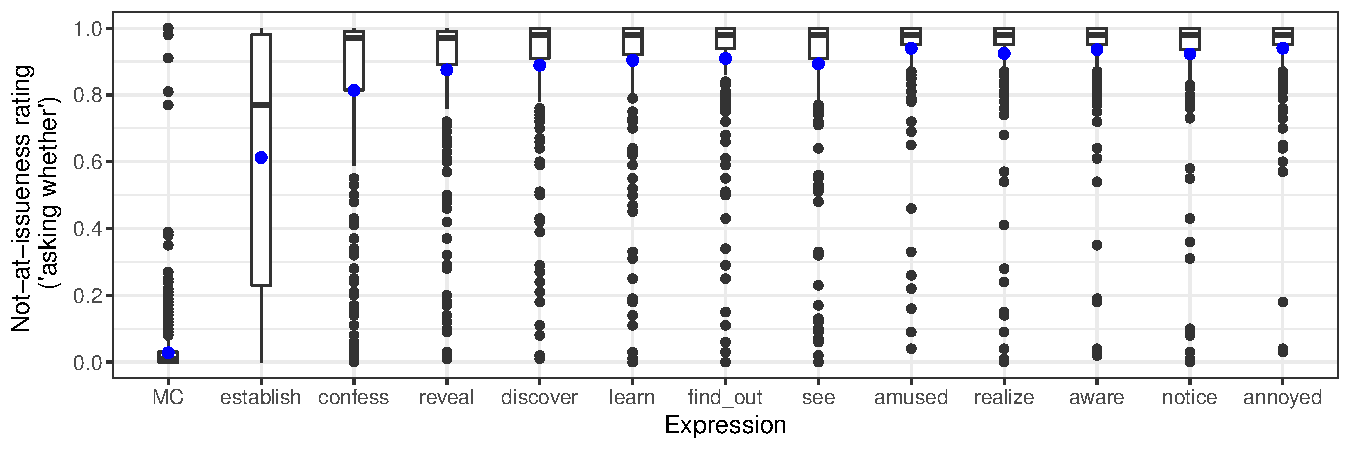
\includegraphics[width=16cm]{../results/exp1b/graphs/boxplot-not-at-issueness-with-MCs}
\label{fig:aimeans-1b}
}

\subfloat[][Boxplot of not-at-issueness ratings in Exp.~2b.]{ 
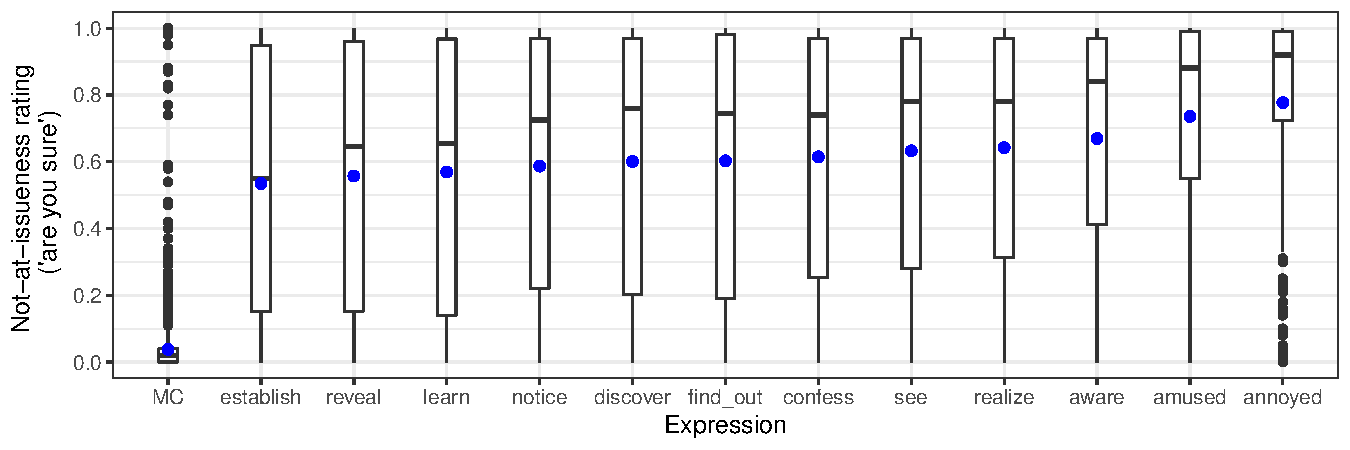
\includegraphics[width=16cm]{../results/exp2b/graphs/boxplot-not-at-issueness-with-MCs}
\label{fig:aimeans-2b}
}

\end{center}
\caption{Not-at-issueness ratings by expression, including main clauses and collapsing across lexical contents, in Exp.~1b (top panel) and Exp.~2b (bottom panel). Grey dots indicate means and notches indicate medians.}
\label{f-ai-b}
\end{figure}

\bibliographystyle{cslipubs-natbib}
\bibliography{bibliography}


\end{document}
